
%%
%% OSDI 2014 Submission requirements
%% 12 pages + plus as many pages as needed for references.
%%
%% Blind reviewing of full papers will be done by the program committee
%% and external review committee, with limited use of outside
%% referees. Authors must make a good faith effort to anonymize their
%% submissions, and they should not identify themselves either explicitly
%% or by implication (e.g., through the references or
%% acknowledgments). Submissions violating the detailed formatting and
%% anonymization rules will not be considered for publication.

% Usenix/OSDI requirements 
\documentclass[10pt,twocolumn]{article}
\usepackage{times}
\usepackage{fullpage}

% added for our purpose
\usepackage{xspace}
\usepackage{url}
\usepackage{upgreek}
\usepackage{comment}
\usepackage{graphicx}
\usepackage{subfig}
\usepackage[normalem]{ulem}
\usepackage[hidelinks]{hyperref}
% name of the product in a funky font
\newcommand{\microsecond}{$\upmu{}$s\xspace}
\newcommand{\ix}{\textsc{ix}\xspace}
\newcommand{\twiddle}{$\sim$}

%%%%%%%%%%%%%%%%%%%%%%%%%%%%%%%%%
% SQUEEZING SPACE

\usepackage[compact]{titlesec}%squeeze

%\newcommand{\myparagraph}[1]{{\bf #1}}
%\newcommand{\myparagraph}[1]{\paragraph{#1}}
%\newcommand{\myparagraph}[1]{{\vspace{5pt}\noindent\bf #1}}
\newcommand{\myparagraph}[1]{{\vspace{3pt}\noindent\bf #1}}

%\addtolength{\parskip}{-5pt}
\addtolength{\abovecaptionskip}{-5pt}
\addtolength{\belowcaptionskip}{-10pt}

%%%%%%%%%%%%%%%%%%%%%%%%%%%%%%%%
% debugging only
\usepackage[usenames,dvipsnames]{xcolor}
\newif\ifcomments
\commentstrue

%% Uncomment the following line to remove comments from text and get an
%% accurate page count.
\commentsfalse

\ifcomments
\newcommand{\edb}[1]{\noindent{\color{Plum} {\bf \fbox{EdB} {\it#1}}}}
\newcommand{\adam}[1]{\noindent{\color{Red} {\bf \fbox{AB} {\it#1}}}}
\newcommand{\christos}[1]{\noindent{\color{Green} {\bf \fbox{CK} {\it#1}}}}
\newcommand{\george}[1]{\noindent{\color{Blue} {\bf \fbox{GP} {\it#1}}}}
\newcommand{\ana}[1]{\noindent{\color{Orange} {\bf \fbox{AK} {\it#1}}}}
%\newcommand{\babak}[1]{\noindent{\color{Purple} {\bf \fbox{BF}} {\it#1}}}
\newcommand{\dm}[1]{\noindent{\color{Red}{\fbox{DM} {#1}}}}
\newcommand{\todo}{\noindent $\triangleright $~}
\else
\newcommand{\edb}[1]{}
\newcommand{\adam}[1]{}
\newcommand{\christos}[1]{}
\newcommand{\george}[1]{}
\newcommand{\ana}[1]{}
\newcommand{\dm}[1]{}
\newcommand{\todo}[1]{}
\fi
\newcommand{\oldcite}[2]{\item #1 ({\small #2})\cite{#2}.}

%%%%%%%%%%%%%%%%%%%%%%%%%%%%%%%%%%%%%%%%%%%%
\begin{document}

%%%%%% TITLE OPTIONS
%\title{\bf Title}
%\title{ Scalability, Quality-of-service, and Energy Proportionality of the IX Domain-Specific Operating System}
%\title{\bf IX: A Dataplane Architecture for \break Event-driven, Web-scale Applications}
\title{\bf IX: A Dataplane Operating System for \break Event-driven, Web-scale Applications}

% author list to be finalized at camera-ready time. 
% placeholder for now. -EdB
%\author{Adam Belay \and Georgios Prekas \and Edouard Bugnion \and Christos Kozyrakis}

\author{Paper \# 136}
\date{}
\maketitle
\thispagestyle{empty}

\begin{abstract}
Lorem ipsum lorem ipsum lorem ipsum lorem ipsum lorem ipsum lorem ipsum
lorem ipsum lorem ipsum lorem ipsum lorem ipsum lorem ipsum lorem ipsum
lorem ipsum lorem ipsum lorem ipsum lorem ipsum lorem ipsum lorem ipsum
\end{abstract}


\section{Introduction}
\label{sec:intro}


\dm{The intro is very buzzword-heavy, which makes a fundamental
  contribution (architecture for super low-overhead networking) sound
  really artifactual.  The term ``web-scale'' does not do us any
  favors.  Yes right now the web and social networking are hot topics,
  but these should be presented as examples of services that can
  benefit from sub-microsecond receive paths.  Our contribution is not
  to fix twitter's or Amazon's problems in 2014.  It is a fundamental
  re-thinking of how to design network APIs for modern NIC hardware,
  which could enable new types of system down the line.}

Web-scale applications such as search, social networking, and
e-commerce platforms, are redefining the requirements on system
software. A single application can consist of hundreds of software
services, deployed on thousands of servers. For example, Amazon
routinely accesses 150 distinct services to render each page requested
by external users~\cite{DBLP:conf/sosp/DeCandiaHJKLPSVV07}. Such
applications need TCP/IP networking stacks that go well beyond the
classical requirements of high streaming performance and moderate
connection scalability. The new requirements include high packet rates
for short messages~\cite{Atikoglu:2012:WAL}, microsecond-level
responses to remote requests with tight tail latency
guarantees~\cite{DBLP:journals/cacm/DeanB13}, and support for hundreds
of thousands of connections with high connection
churn~\cite{nishtala2013scaling}. It is also desirable to be elastic
in resource usage, allowing other applications to use any available
cores and memory in a shared cluster~\cite{nishtala2013scaling} or
enabling cost reduction through power
management~\cite{DBLP:journals/computer/BarrosoH07}.


% \christos{1-2 paragraphs on how mainstream approaches fail many 
% of these requirements. A trimmed down version of what is shown below. }
% At massive scale, these interactions constrain applications.  For
% example, latency considerations force Facebook to restrict the number
% of sequential data accesses to fewer than 150 per rendered web
% page~\cite{rumble2011s}.  Also at Facebook, connection scalability
% limitations have led the deployment of a UDP-based memcached service
% tier~\cite{nishtala2013scaling} for \texttt{get} operations, which
% therefore forgoes all of the benefits of the standard TCP-based model.
% To ensure the reliable application of \texttt{put} operations, the
% system relies on in-network TCP-proxies to aggregate requests, which
% introduces complexity and latency in the architecture.

% In a recent keynote, \edb{too personal?}Google's Luiz Barroso identified three additional challenges
% for applications that must process large amounts of data in little
% time: energy-proportionality, tail-tolerance, and microsecond
% computing~\cite{luiz-isscc}.
% Energy-proportionality~\cite{DBLP:journals/computer/BarrosoH07}
% requires systems to perform with a high degree of energy-efficiency,
% typically measured in transactions / Watt, across all typical levels
% of load on the system, and not only at saturation. Tail
% tolerance~\cite{DBLP:journals/cacm/DeanB13} describes the emerging
% systems-building discipline that aims to deliver predictable response
% times in a distributed system.  Finally, the microsecond computing
% challenge describes the need to minimize the latency of interactions
% within a datacenter: even though existing transmission and switching
% technologies allow for microsecond-level messaging between any two
% nodes in a datacenter, a combination of protocol processing, interrupt
% delivery, and operating system overheads generally increase the
% latency by two orders of magnitude.  Although each challenge is
% non-trivial in itself, these challenges must be handled
% simultaneously.  Unfortunately, techniques that improve one metric are
% often at odds with another metric.  For example, dynamic voltage
% scaling techniques improve energy-proportionality for batch
% applications~\cite{DBLP:conf/asplos/DelimitrouK14}, but at the
% expense of latency.  Similarly, batching techniques such as interrupt
% coalescing improve performance at the expense of average and tail
% latency~\cite{missing}.

% \dm{Bad to rely on ``conventional wisdom'' without citation, but we
%   can reasonably quantify such overheads ourselves to state a fact.
%   E.g., ``Currently the only option for meeting XXX performance
%   requirement is to bypass the kernel[cite], with the following
%   disadvantages\ldots''} 
The conventional wisdom is that there is a fundamental mismatch
between the requirements of web-scale workloads and existing
implementations of TCP/IP in commodity operating
systems. Consequently, many proposed solutions bypass the OS and
implement the networking stack in
user-space~\cite{jeong2014mtcp,Kapoor:2012:CPL,openonload,marinos2013network,Thekkath:1993:INP}. Some
systems go one step further by also replacing TCP/IP with RDMA in
order to offload protocol processing to Infiniband network
adapters~\cite{DBLP:conf/sosp/OngaroRSOR11,Jose:2011:MDH,mitchell:rdma,dragojevic14farm}. While
kernel bypass eliminates context switch overheads, on its own it does
not eliminate the difficult tradeoffs between high packet rates and
low latency or the challenges of managing large numbers of
connections. Moreover, user-level networking suffers from lack of
protection. Application bugs and crashes can corrupt the networking
stack and impact other workloads.

% Christos: I have decided to postpone the discussion of all other
% alternatives in section 2. Simplifies the message in the intro
% The conventional wisdom is that these problems are rooted in a
% mismatch between existing commodity operating systems, existing
% network protocols, and the unique requirements of web-scale
% applications.  Consequently, the proposed solutions generally involve
% either: (i) improving the operating system's implementation and
% interface~\cite{DBLP:conf/eurosys/PesterevSZM12,han2012megapipe}; (ii)
% replacing network-level connections with
% datagrams~\cite{nishtala2013scaling}; (iii) offloading connection and
% protocol processing to a specialized hardware adapter, e.g, the
% RAMcloud~\cite{DBLP:conf/sosp/OngaroRSOR11} key-value store relies on
% RDMA~\cite{rdma-user-manual} to achieve 5~\microsecond latency; (iv)
% bypassing the operating system and implementing the protocol stack in
% user-space~\cite{jeong2014mtcp}; (v) merging the application logic
% directly within a software data plane, as is commonly done in
% middleboxes such as firewalls~\cite{missing},
% load-balancers~\cite{missing}, and software
% routers~\cite{DBLP:journals/tocs/KohlerMCJK00,DBLP:conf/sosp/DobrescuEACFIKMR09};
% or even (vi) replacing the general-purpose hardware with a specialized
% FPGA implementation dedicated to serving a single, simple workload
% such as memcached~\cite{DBLP:conf/fpga/ChalamalasettiLWARM13}.

% \christos{This is where we bring up the design principles of IX:
%   separation data/control plane; native zero-copy event-oriented API; 
% data-plane architecture that runs to completion; design for multi-core
% and multi-queue. Probably two paragraphs}

\dm{Again, this makes it sound narrow.  Phrase in a more fundamental
  way.  Point is that currently people must achieve a delicate $n$-way
  balance between throughput, latency, protection/robustness,
  complexity, number of machines/power consumption, etc.  \ix shows it
  doesn't have to be this way; we can have our cake and eat it, too,
  if we architect better systems around improved APIs.} 

We propose \ix, an operating system designed specifically to meet the
networking requirements of event-driven, web-scale applications.  Its
architecture builds upon the lessons from high performance
middleboxes, such as firewalls, load-balances, and software
routers~\cite{DBLP:journals/tocs/KohlerMCJK00,DBLP:conf/sosp/DobrescuEACFIKMR09}. \ix
separates the control plane, which is responsible for basic kernel
functionality such as provisioning and scheduling, from the dataplanes
which run the networking stack and application logic. However, \ix
uses hardware virtualization~\cite{DBLP:journals/computer/UhligNRSMABKLS05} to isolate the control plane from the
dataplanes and offer
the same protection model as commodity operating systems. In our
implementation, the control plane runs on a vanilla Linux kernel and
the dataplanes use Dune to run \ix as protected, library-based
operating systems~\cite{belay2012dune}. \adam{new:} Dune makes this
possible by directly exposing hardware protection mechanisms
using virtualization hardware.

\ix provides a native, zero-copy API that explicitly exposes network
flow-control to applications.  This API enables dataplanes to optimize
for both bandwidth and latency by processing a bounded batch of
packets to completion.  Each dataplane executes all the pipeline
stages for TCP/IP processing for the batch in kernel mode, followed by
the associated application processing in user mode. This approach
amortizes API overheads and improves both instruction and data
locality.  \ix is also optimized for synchronization and coherence
free execution on multi-core systems. It uses multi-queue network
adapters (NICs) and receive-side scaling (RSS)~\cite{url:rss} to
implement flow-consistent hashing of incoming traffic to distinct
hardware queues. Each dataplane instance exclusively controls a set of
these queues and runs the networking stack and a single application,
such as a webserver or a distributed caching server. Moreover, the \ix
API and companion user-level library meet the commutativity
rule~\cite{DBLP:conf/sosp/ClementsKZMK13}, eliminating multi-core
synchronization in the common case operation. The \ix user-level
library includes an interface nearly identical to the popular
\texttt{libevent} library~\cite{provos2003libevent}, providing
compatibility between \ix and a wide range of existing applications.

\dm{The above paragraph does a reasonable job of describing what's
  new.  But it might be worth another paragraph addressing why now
  Basically there's a fundamental question of granularity here.  E.g.,
  page sizes have been 4--8K since machines had less than a Megabyte
  of DRAM\@.  Schedulers have been designed under the premise of more
  applications than CPUs.  Network APIs were designed when packet
  inter-arrival times were many times the system call/interrupt
  latency.}

\dm{Another point to add is that the breadth of OS APIs has made it
  virtually impossible to deploy clean-slate operating systems,
  despite possibly huge performance gains from radically different IO
  architectures.  Fortunately, the performance-critical IO functions
  are a small subset of the garbage can of system calls required for
  setup, initialization, and configuration.  Hence, a big contribution
  is showing how we can completely rearchitect the IO path while
  retaining a high degree of source code compatibility and remaining
  compatible with existing system configuration and management tool.}

% \ix addresses the C10M problem through a careful separation of the
% control plane and dataplane functions.  The control plane consists of a
% vanilla Linux deployment running the Dune
% framework~\cite{belay2012dune}. 

% The dataplane is a special-purpose library operating system that
% directly controls hardware I/O queues, runs the networking stack, and
% generates the event callbacks of the application.  Each dataplane
% instance exclusively controls a set of hardware I/O queues, and runs a
% single application, e.g. a web sever listening to \texttt{:80} and
% \texttt{:443}.  Unlike kernel-bypass approaches and middlebox designs,
% \ix provides memory protection.  Like these designs however, \ix
% offers a zero-copy solution both directions, eliminating all packet
% copy overheads.


% We introduce \ix, a specialized system software solution built for
% event-driven applications, including applications built for the
% libevent framework~\cite{provos2003libevent}.  \ix is designed to meet the
% challenge of the C10M problem~\cite{theC10Mproblem}: for a given
% server, scale to 10 million concurrent TCP connections, saturate one
% or multiple 10 GbE interfaces, and deliver 10~\microsecond latency
% (mean), with an additional latency jitter of not more than an extra
% 10~\microsecond.

% The primary contributions of the \ix design are: (i) the combined use
% of commodity OS and virtualization hardware to separate control from
% data plane in a protected networking stack; (ii) a run-to-completion
% execution model with cooperating, untrusted applications; (iii) a
% bounded, adaptive batching mechanism that provides both low-latency
% and high throughput; (iv) an implementation carefully optimized for
% multi-core scalability. 

We compare \ix against Linux 3.11.10 and mTCP, a state-of-the-art
user-level TCP stack~\cite{jeong2014mtcp}.  On networking
microbenchmarks that are either latency-sensitive, require a high TCP
connection churn, or manage a large number of concurrent connections,
\ix outperforms Linux by an order of magnitude, and mTCP by up to
2.5x.  \ix even scales to 4x10GbE configuration, using a single
multi-core socket.  Our evaluation with memcached, a real-world,
massively deployed key-value store, shows that \ix improves upon Linux
by 1.8x-2.7x in terms of throughput at a given 95th percentile latency
bound, as it can reduce kernel mode processing from $>80\%$ with Linux
to $<33\%$ with \ix.

\ix demonstrates that, by revisiting the networking APIs and taking
advantage of modern NICs and multi-core chips, we can design systems
that achieve high throughput \underline{and} low latency
\underline{and} high connection counts \underline{and} robust
protection. It also shows that, by separating the the small subset of
performance-critical I/O functions from the rest of the kernel, we can
design systems with radically different I/O architectures and achieve
large performance gains, while retaining compatibility with the huge
set of APIs and services provided by a modern OS.


% \christos{I prefer to enumerate the main design principles and the
%   list impressive numbers towards the goals rather than come up with
%   another contribution list that is repetative}
% The primary contributions of this paper are as follows:

% \begin{itemize}

% \item  the use of Linux and Dune as a mechanism to separate the control-plane from the dataplane in web-scale applications;

% \item the design and implementation of \ix, a library operating system
%   organized as a protected dataplane with zero-copy specifically
%   designed to support event-driven applications;

% \item an evaluation of \ix that shows that we meet the C10M challenge;
%   despite the conventional wisdom, this is achieved through a
%   specialized kernel (organized as dataplane);

% \item the evaluation of \ix that shows that it outperforms the
%   state-of-the-art userlevel stack by \edb{3x?} or more for all
%   micro-benchmarks and real-world applications such as memcached;

% \item XXX

% \end{itemize} 

\christos{Eliminate if we don't have space} The rest of the paper is 
organized as follows. \S \ref{sec:motivation} motivates the need
for a new OS architecture for web-scale applications. \S\ref{sec:design} and \S\ref{sec:impl} present the design principles and
implementation of \ix. \S\ref{sec:eval} presents the
quantitative evaluation.\S\ref{sec:disc} and \S\ref{sec:related} discuss future and related work.








\section{Background and Motivation}
\label{sec:motivation}

Our work focuses on identifying the mismatch and opportunities for
improvement between commodity operating systems and a large, but
well-defined, class of relevant applications.
%  In this section, we
% first define the class of applications in our focus
% (\S\ref{sec:motivation:web}), then describe the system software
% challenges associated with that class of applications
% (\S\ref{sec:motivation:challenges}), and identify an alternative model
% -- the dataplane -- which addresses these challenges
% (\S\ref{sec:motivation:dp}.

\subsection{Event-driven, Web-scale Applications}
\label{sec:motivation:web}

Modern web-scale applications include interactive services such as
search, social networking, webmail and instant messaging, online maps,
automatic translation, software as a service (SaaS), and e-commerce
platforms.  We have come to expect that these services provide
millions of users with instantaneous, personalized, and contextual
access to petabytes of data.  For example, the Google search engine
updates query results interactively as the user types, predicting the
most likely query, performing the search and showing the results
within a few tens of milliseconds~\cite{DBLP:journals/cacm/DeanB13}.

Internally, such applications use a service-oriented architecture and
consist of tens of distinct, well-defined services such as
load-balancing and http proxies, web and application serving, content
distribution and streaming, memory caching, queuing services,
relational databases and object
storage~\cite{Alonso:2010:WSC,Eriksen:2013:YSF}. \christos{what is the
  authoritative ref for SOA?} Collectively, these services occupy
hundreds to thousands of servers connected through high-speed
networking. Different services are routinely implemented using
different programming languages and paradigms, but are connected
through a unifying framework for RPC, serialization, service
discovery, and logging \cite{protocolbuffers, thrift, fingale,
  others}. An incoming request from an external user leads to tens to
hundreds of internal requests across the various services, with some
requests issued sequentially due to dependencies in application logic,
while other requests are issued in a parallel, fan-out manner.
% In addition, web-scale applications also rely on massive,
% batch-oriented services that prepare the data for interactive serving
% (e.g., the search engine crawlers), identify patterns and behavior
% from the massive data sets and the users' behaviors via machine
% learning~\cite{missing}.

Each node for these services responds to external requests such as new
incoming connections, data requests from existing connections, or
replies to requests made to a downstream service.  The most efficient
implementations today use event-driven framworks in which the service
logic interacts with the framework exclusively via non-blocking
calls. This is in contrast with the classic thread-oriented
programming paradigm, in which sessions are divided among a large pool
of (kernel) threads, which block while waiting for incoming traffic or
outstanding replies. For example, the event-oriented nginx HTTP server
and proxy~\cite{reese2008nginx} outperforms the thread-oriented Apache
server~\cite{misc:apache}.

High-level libraries simplify the development of event-driven
applications~\cite{provos2003libevent,libev,libuv}.  For example, the
popular \texttt{libevent} library~\cite{provos2003libevent} provides a
level of abstraction that exposes the paradigm to applications running
on top of Linux, *BSD, and Windows.  Many web-scale applications, such
as memcached~\cite{missing}, are built on top of libevent.  Others
such as Nginx and node.js are built using similar frameworks.


\subsection{Main Requirements}
\label{sec:motivation:challenges}

Although the event-based paradigm has several system-level benefits,
such as lower context switching rates, its use in web-scale
applications poses many unique challenges to system software:

{\bf High packet rates:} The requests and, often times, the replies
between services in web-scale applications are quite small. In the
memcached service at Facebook, for example, the vast majority of
requests use keys shorter than 50 bytes and involve values shorter
than 500 bytes~\cite{Atikoglu:2012:WAL}. As a result, each service
node must ideally scale to extremely high packet rates, measured in
millions of packets per second on 10 GbE or 40 GbE network interfaces (NICs).
In such conditions, common hardware optimizations found in network
interfaces, such as TCP segmentation and large receive offloading,
have a marginal impact on performance. 

{\bf Micro-second latency:} To enable rich interactions between a
large number of services in a web-scale application without impacting
the overall latency experienced by the user, it is essential to
minimize the latency for each service
request~\cite{luiz-isscc,Rumble:2011:TLL}. Today's networking
technologies allow for one-way communication across a large-scale
datacenter within a few \microsecond : 3~\microsecond latency across
a pair of 10 GbE NICs~\cite{cisco-sereno}, one to five switch
crossings with cut-through latencies of a few hundred $ns$ each, and
propagation delays of 500 $ns$ for 100 meters distance. Unfortunately,
system software is designed to operate at a totally different
timescale. Interrupt coalescing used to improve throughput, queuing
latency due to device driver processing intervals, and protocol
processing of incoming packets without necessarily immediately
scheduling the receiving application frequently add several $ms$ of
latency to to remote procedure calls (see measurements in Section
\ref{sec:eval}).

% As a result, the remote procedure call latency observed by application
% software is one to two orders of magnitude greater than the intrinsic
% latency.  For example, we measure the average NetPIPE latency between
% two vanilla Linux servers with Intel XXX NICs at XXX\microsecond, when
% in fact such communication is possible in only XXX\microsecond (see
% \S\ref{missing}).

These issues compound when considering the long tail of the latency
distributions of RPCs across thousands of
servers~\cite{DBLP:journals/cacm/DeanB13}. Although tail-tolerance is
actually an end-to-end challenge, the system software stack plays a
significant role in exacerbating the problem~\cite{Leverich:RHSU:2014}.
Protocol-processing techniques that reduce latency to \microsecond in
the average, but do no improve 95th or 99th percentile latency are
unlikely to result into end-to-end application gains.

{\bf Connection scalability:} For applications that use thousands
multi-core servers, it is desirable to efficiently support both a
large number of concurrent connections per server, as well as high
churn in these connections.  Ideally, the only limitation to a
server's concurrent connection count should be its memory capacity and
the packet rate and tail latency should be independent of the nunber
of concurrent connections or the rate of churn.
 
Connection scalability has been a historical challenge for commodity
operating systems, reaching 10,000 concurrent connections a decade
ago~\cite{theC10Kproblem} and exceeding one million connections
today~\cite{theC10Mproblem}. For example, the nature of all-to-all
communication between Facebook's application and memcached servers
made it impractical to use TCP sockets between these two tiers,
resulting in deployments that use UDP datagrams for \texttt{get}
operations and an aggregation proxy for \texttt{put}
operations~\cite{nishtala2013scaling}.

{\bf Resource elasticity:} The load of web-scale applications varies
significantly due to diurnal patterns and unexpected spikes in user
traffic. Ideally, each service node will use the minimum amount of
resources (cores, memory, or IOPS) needed to satisfy packet rate and
tail latency requirements at any point in time. The remaining
resources can be allocated to other applications in a shared
datacenter (e.g., background
analytics)~\cite{Hindman:2011:MPF,DBLP:conf/asplos/DelimitrouK14,Leverich:RHSU:2014}
or placed into low power modes in order to achieve energy
proportionality~\cite{DBLP:journals/computer/BarrosoH07}.
\christos{keeping this simple since we will not do much in this paper}

% Datacenters for web-scale applications are
% essentially built today using thousands of commodity Xeon-class
% processors that draw hundreds of Watts each.  The dimension of each
% building block -- number of sockets, cores, DRAM, disk capacity, IOPS
% and bandwidth, and networking bandwidth -- are largely determined by
% architectural trends.  Ideally, applications would only consume
% resources (incl. energy) that are proportional to their current load.
% Unfortunately, mapping such applications efficiently onto the
% scale-out model remains an open challenge~\cite{missing} as it requires
% a combination of cluster-wide, and machine-local resource management,
% workload placement and rebalancing techniques~\cite{missing,missing}.

{\bf Security and protection:} Finally, as multiple foreground and
background services share multi-core servers even in private
datacenters~\cite{Schwarzkopf:2013:OFS,DBLP:journals/cacm/DeanB13},
there is need for isolated protocol stacks. For single-tenant
deployments where all services are administered by the same
organization, the use of TCP-based protocol running with commodity
kernels such as Linux largely addresses the problem.  Challenges
emerge when the networking stack is lifted into the user-space and
application bugs can corrupt the networking stack and impact other
services.


\subsection{Current Approaches}
\label{sec:motivation:current}

\christos{If we leave this here, it is essentially related work. It
  needs to be beefed up and will overlap with the one at the end. I
  suggest we inline the critique to current approaches in the two
  previous section. In 2.1, we add a paragrah that lists the main
  approarch. Then as we review requirements, we inline in each
  paragraph how some current approaches fail it. }

The conventional wisdom is that these challenges are rooted in a
mismatch between existing commodity operating systems, existing
network protocols, and the unique requirements of web-scale
applications.  Indeed, with today's technology, commodity Xeon
processors support 8-10 cores with dedicated L1 caches, between 16-40
hyperthreads, up to 50 Gbps of PCIe bandwidth \christos{Intel E5 chips
  have 24GBytes/sec PCIe bandwidth per socket}, and NIC that transfer
frames in a few \microsecond.  Unfortunately, the distinct nature of
web-scale applications prevents them from saturating the hardware.
Different approaches have been proposed to address each a subset of
these challenges:

\paragraph{Running the networking stack in user-space.}  

Approaches such as OpenOnload~\cite{openonload} or
mTCP~\cite{jeong2014mtcp} run the entire networking stack in
userspace, which are designed to offer load-latency communication
(e.g. OpenOnload) or connection scalability (e.g. mTCP), at the
expense of protection.  mTCP's design has the TCP stack running on
dedicated hyperthreads which synchronizes at relatively coarse grain
with the application. Although tail latency can be bounded, the focus
is measured at ms-scale rather than \microsecond-scale.

\paragraph{Alternatives to TCP.}

Low-latency key-value stores such as
RAMcloud~\cite{DBLP:conf/sosp/OngaroRSOR11} rely on kernel-bypass and
RDMA to offload all protocol processing on dedicated Infiniband Host Channel
Adapters.  Using standard hardware and networking fabrics, Facebook's
deployment of memcached uses UDP to avoid any connection scalability
limitations.  Even though UDP itself is running in the kernel, the
responsibilities of congestion management and flow control and
entrusted into applications.

\paragraph{Alternatives to POSIX API.}

MegaPipe~\cite{han2012megapipe} replaces the POSIX API with
lightweight sockets implement by in-memory command rings.  This
substantially reduces software overheads and substantially increases
packet rates.  The pragmatic use of the operating system's TCP stack
and interrupt model presents any microsecond-computing solution.

\paragraph{Enhancements to the OS.}

Operating system modifications tradeoff superior ease of deployability
(and quite frankly, pragmatism in terms of production use) even though
the improvements might be more incremental.
Affinity-Accept~\cite{DBLP:conf/eurosys/PesterevSZM12} improves the
affinity of incoming and outgoing network processing by considering
the affinity of flows to core and controlling the NIC hardware.  Linux
\texttt{SO\_REUSE} allows multi-threaded applications to accept
incoming connections in parallel.  Although such approaches minimize
communication between core, they do not eliminate them.  The lack of
commutativity~\cite{DBLP:conf/sosp/ClementsKZMK13} in the POSIX socket
API implies that cross-core communication is necessary whenever a
connection is accepted or closed.  When microsecond latencies are
irrelevant, such as Internet-facing communication services, properly
tuned stacks can support millions of concurrent connections in
production~\cite{whatsapp-2mil}.  

\section{\ix Design Approach}
\label{sec:design}

% We now present the fundamental design principles of a dataplane
% architecture designed to run untrusted, event-driven applicatxions,
% and designed to address the specific scalability challenges of
% today's web-scale applications.

The first three requirements of \S\ref{sec:motivation:challenges} --
high packet rate, microsecond latency, and connection scalability--
are not unique to web-scale applications.  These requirements have
been addressed in the design of middleboxes such as firewalls,
load-balancers, and software
routers~\cite{DBLP:journals/tocs/KohlerMCJK00,DBLP:conf/sosp/DobrescuEACFIKMR09};
by integrating the networking stack and the application into a single
\emph{dataplane}. The two remaining requirements -- resource
elasticity and protection -- are not addressed in middleboxes because
they are single-purpose systems, not exposed directly to users.

% As for the other two remaining aspects -- resource elasticity and
% security and protection --, middleboxes provide fewer insights: since
% each middlebox typically performs a single function, resource
% elasticity and proportionality is less of a direct concern.  They are
% traditionally deployed and maintained using an embedded paradigm in
% which the entire stack -- operating system, applications and utilities
% -- is packaged as single blob.  As such, the security and protection
% model is not directly exposed to users.

Dataplanes differ from traditional OS designs in two fundamental
ways. First, they are designed to \emph{run each packet to
  completion}. All network protocol and application processing for a
packet is done before moving on to the next packet.  In contrast, a
commodity OS decouples protocol processing from the application itself
in order to provide scheduling and flow control flexibility.  For
example, a commodity OS relies on device and soft interrupts to
context switch from application to protocol processing. Similarly, the
kernel's networking stack will generate a TCP \texttt{ACK} and slide
its receive window even when the application is not consuming data, up
to an extent. Second, dataplanes are designed to operate in a
\emph{flow-consistent, coherence-free} manner.  Network flows are
distributed into distinct queues via receive-side scaling
(RSS)~\cite{url:rss} and the common case packet processing requires no
synchronization or coherence traffic between cores.

% Flow-consistency distributes flows
% into distinct queues based on a L4-hash; this is routinely supported
% in network CPUs used in middleboxes (e.g., ~\cite{cavium-octeon}) as
% well as commodity NIC via Receive Side Scaling (RSS)~\cite{missing}.

Building upon the lessons from middleboxes, we design \ix to answer
the following question: {\it \ana{how} can the dataplane architecture be
  efficiently extended to support untrusted, event-driven applications
  and satisfy simultaneously the five requirements of
  \S\ref{sec:motivation:challenges}?}  The answer relies on the
following key design principles:


\myparagraph{Separation and protection of control and data plane:} 
% Software dataplanes are designed to operate on flows, not to
% provision resources or manage them in an elastic and proportional
% manner.
Our design separates the control function of the kernel, responsible
for resource configuration, provisioning, scheduling, and monitoring,
from the dataplane, which runs the networking stack and application
logic.  Like a conventional OS, the control plane multiplexes and
schedules resources among dataplanes, but in a coarse-grained manner
in space and time: cores are dedicated to applications until revoked,
memory is allocated at large page granularity of physical memory;
hardware queues are exclusively assigned to a single dataplane until
explicitly revoked.  The separation allows us to consider \george{double word?} radically
radically I/O APIs and implementations in the dataplane, while
retaining full compatibility with a modern OS like Linux.  Similar to
Exokernel~\cite{DBLP:conf/sosp/EnglerKO95}, each dataplane runs a
single application in a single address space.

 % of  using library operating systems~\cite{DBLP:conf/sosp/EnglerKO95}.

\myparagraph{Native zero-copy API with explicit flow control:} We do
not expose or emulate the POSIX API for networking.  Instead, the
dataplane and the application communicate asynchronously with each
other via messages stored in
memory~\cite{rizzo2012netmap,han2012megapipe}.  The API meets the
commutativity rule~\cite{DBLP:conf/sosp/ClementsKZMK13} and allows for
a true zero-copy operation in both directions. The dataplane and
application cooperatively manage the message buffer pool. Incoming
packets are mapped read-only into the application, which may hold onto
message buffers and return them to the dataplane at a later point.
The application sends to the dataplane scatter/gather lists of memory
locations for transmission but, since contents are not copied, the
application must keep the content immutable until the peer
acknowledges reception. The kernel implements all flow control
mechanisms and may trim transmission requests that exceed the
available size of the sliding window.  Essentially, the API directly,
but safely, exposes flow control to applications.


% \myparagraph{Explicit flow control:} The API supports a zero-copy,
% non-blocking API that directly, but safely, exposes flow control to
% applications. The application may send to the dataplane scatter/gather
% lists of memory locations for transmission.  The kernel trims requests
% that exceed the available size of the sliding window. As the contents
% are not copied, the application must further keep the content
% immutable until the peer later acknowledges reception.  Although the
% kernel implements all flow control mechanisms, it does not introduce
% additional buffering or abstraction mechanisms, allowing applications
% to make appropriate policy decisions.


\myparagraph{Run to completion with adaptive batching:} Our dataplane
runs to completion all pipeline stages needed to receive or transmit a
packet, interleaving protocol processing (kernel mode) and application
logic (user mode) as needed. Hence, there is no need for intermediate
buffering between pipeline stages or between the application logic and
the TCP/IP stack. Run to completion has been previously proposed to
address receive livelock within the OS~\cite{receivelivelock}. We
extend it to both kernel and user-level, which eliminates interrupts
and improves data locality throughout the common case packet
processing.

Batch processing minimizes instruction overheads and increases
instruction locality. Previous proposals batch only at the API level
in order to amortize system call
overhead~\cite{jeong2014mtcp,han2012megapipe,soares2010flexsc}. We
execute every pipeline stage on a small batch of packets or commands
to fully amortize instruction caching effects and the overhead of PCIe
transfers. To minimize the impact on latency, we perform adaptive
batching as follows: (i) we never wait to batch requests and batching
only occurs in the presence of congestion; (ii) we set an upper bound
on batches of 128 packets, a value experimentally determined to
effectively amortize startup overheads.


% Christos; this is essentially the other half of the "expose flow
% control to applications". oh well...
The combination of adaptive batch processing and zero copy means that
queues for incoming packets can build up only at the NIC edge, before
packets are processed by the dataplane. \ana{Emphasize that we are not
  wasting resources on packets that might have to be dropped; drop
  early at the NIC if can't handle.  Citation for Mogul and
  Ramakrishnan could go here.} The networking stack sends
acknowledgments to peers only as fast as the application can process
them. Any slowdown in the application processing rate quickly leads to
shrinking windows in peers. The dataplane also monitors queue depths
at the NIC edge and signals the control plane to allocate additional
resources for the dataplane (more hardware threads, increased clock
frequency), notify peers explicitly about congestion (e.g., via
ECN~\cite{ramakrishnan2001addition}), and make policy decisions for
congestion management (e.g., via
RED~\cite{DBLP:journals/ton/FloydJ93}).

% \myparagraph{Buffering at the NIC edge:} The consequence of adaptive
% batching is the buildup of queues at the NIC edge before the packets
% are processed by the dataplane.  Because of the dataplane's design,
% congestion occurs only at the NIC edge.  In effect, the NIC edge acts
% like the last-hop buffer in the network.  This has an additional
% benefit in terms of flow control, as the networking stack sends
% acknowledgments to peers only as fast as the application can process
% them.  Congestion in the NIC edge therefore leads to shrinking windows
% in peers, and flow control.


% Like switches and routers, the NIC edge can
% monitor queue depths to detect congestion, signal the control plane to
% allocate additional resources (more hardware threads, increase clock
% frequency) for the dataplane, notify explicitly flow sources of
% congestion (e.g., via ECN~\cite{ramakrishnan2001addition}), and finally make
% policy decisions when it is necessary to manage congestion (e.g., via RED~\cite{DBLP:journals/ton/FloydJ93}).

\begin{figure}
\begin{centering}
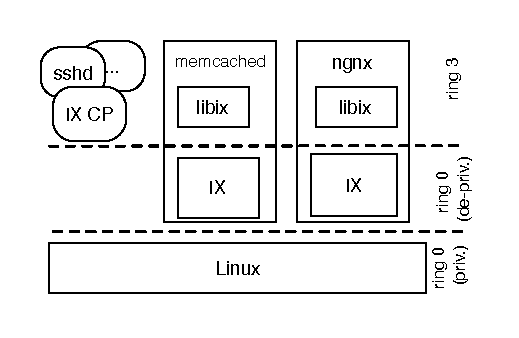
\includegraphics{figs/cp-dp.eps}
\centering\caption{Protection and separation in \ix.}
\label{fig:cp-dp}
\end{centering}
\end{figure}





\myparagraph{Flow consistent, coherence-free processing:} We use
multi-queue NICs with RSS support to provide flow-consistent hashing
of incoming traffic to distinct hardware queues. Each queue is served
by a single hardware thread all the way to the application layer,
eliminating the need for synchronization and cache coherence traffic
between cores. Similarly, memory management is organized in distinct
pools for each hardware thread. The absence of a socket layer
eliminates the issue of the shared file descriptor namespace in
multithreaded
applications~\cite{DBLP:conf/sosp/ClementsKZMK13}. Hence, our design
scales well with the increasing number of cores in modern servers. Our
approach does not restrict the memory model for
applications. Application logic can take advantage of coherent, shared
memory to exchange information and synchronize between cores.






\section{\ix Implementation}
\label{sec:impl}

\begin{table*}[t]
\centering
\begin{small}
\begin{tabular}{|l|l|l|}
\hline
\multicolumn{3}{|c|}{{\bf System Calls (batched)}} \\
\hline
connect &             cookie, dst\_IP, dst\_port		& Opens a connection\\
accept &              handle, cookie				& Accepts a connection\\
sendv &               handle, scatter\_gather\_array		& Transmits a scatter-gather array of data\\
recv\_done &          handle, bytes\_acked			& Advances the receive window and frees memory buffers\\
close &               handle					& Closes or rejects a connection\\
\hline  \hline
\multicolumn{3}{|c|}{{\bf Event Conditions}} \\
\hline
{\bf Type} &           {\bf Parameters}  &
{\bf Description}\\
knock  &               handle, src\_IP, src\_port		& A remotely initiated connection was opened \\
connected &            cookie, outcome				& A locally initiated connection finished opening \\
recv &                 cookie, mbuf\_ptr, mbuf\_len		& A message buffer was received \\
sent &                 cookie, bytes\_sent, window\_size	& A send completed and/or the window size changed \\
dead &                 cookie, reason				& A connection was terminated \\
\hline
\end{tabular}
\caption{\ix system calls and event conditions API. 
}
\label{tbl:api}
\end{small}
\end{table*}



We now describe the \ix prototype.  The current implementation uses
the VT-x features available on all x86-64
servers~\cite{DBLP:journals/computer/UhligNRSMABKLS05}. However, it can
be ported to any architecture with virtualization support, such as ARM
and Power.

% We start
% with an overview of the \ix kernel (\S\ref{sec:impl:kernel}), describe
% the environment surrounding \ix (\S\ref{sec:impl:env}), and how \ix is
% implemented as a coherency-free kernel (\S\ref{sec:impl:cohfree}).


%the benefits of having \ix run as a guest
%operating system (\S\ref{sec:impl:guest}), its native API at the
%kernel/user boundary (\S\ref{sec:impl:api}), the implementation of the
%networking stack (\S\ref{sec:impl:stack}), the implications on
%congestion management and flow control (\S\ref{sec:impl:net}), the
%benefits and consequences of coherence-free execution
%(\S\ref{sec:impl:cohfree}), and finally our approach to compatibility
%(\S\ref{sec:impl:libix}).

\subsection{Overview}
\label{sec:impl:overview}

Fig.~\ref{fig:cp-dp} presents the \ix architecture, including the
control plane, a number of dataplanes, and applications. The hardware
environment includes one or more multi-queue NICs with RSS support and
a multi-core server.

The \ix control plane consists of the full Linux kernel and
\texttt{IXCP}, a user-level program. The Linux kernel initializes PCIe
devices, such as the NICs, and provides the basic mechanisms for
resource allocation to the dataplanes, including cores, memory, and
network queues. Equally important, Linux provides system calls and
services that are necessary for compatibility with a wide range of
applications, such as file system and signal support. \texttt{IXCP}
monitors resource usage and dataplane performance and implements
resource allocation policies. The development of efficient allocation
policies involves understanding difficult tradeoffs between dataplane
performance, energy proportionality, and resource sharing between
co-located applications as their load varies over
time~\cite{Leverich:RHSU:2014,Lo:2014:TWE}. We leave the design of
such policies to future work and focus this paper on the \ix dataplane
architecture.

We run the Linux kernel in VMX root ring 0, the mode typically used to
run hypervisors in virtualized
systems~\cite{DBLP:journals/computer/UhligNRSMABKLS05}. We use the
Dune system within Linux to enable dataplanes to run as library-based
OSes in the VMX non-root ring 0, the mode typically used to run guest
kernels in virtualized systems~\cite{belay2012dune}. % \ana{Elaborate on
% role of Dune?}
Finally, applications run VMX non-root ring 3. This
approach provides dataplanes with direct access to hardware features,
such as page tables and exceptions, and provides full protection
between the control plane, dataplanes, and untrusted user
code. %\christos{should we explicitly say that most web-scale apps are
%  deployed without VMs so taking over VMX is not a problem?}\edb{not needed}

% \myparagraph{Separation and protection of control and data plane:}
% Each \ix instance and its applications runs as a distinct Dune process
% while control plane functions, including the control and monitoring of
% dataplane, is performed by scripts and daemons of the host
% environments.  This provides protection between control and
% dataplanes. Within each dataplane, \ix further protects itself from
% the untrusted application through virtual memory and by running it at
% userlevel.

% Section Move to the discussion session or future work
% \myparagraph{Elasticity policies:} In contrast to the mechanisms,
% which are generic, different policies can be envisioned to meet
% different use cases and optimization functions.  If neither energy
% proportionality or server consolidation is of any concern, the control
% plane can obviously launch a single dataplane instance configured with
% the maximal available physical resources.  In more realistic
% scenarios, the dataplane is ``right-sized'' to meet its service-level
% agreements with minimal resource allocations.  The control plane can
% further dynamically add or revoke CPUs from a dataplane instances,
% e.g., when the dataplane signals some sustained congestion or
% violation of its service-level agreements, or conversely when the
% allocated CPU resources are underutilized.


Each \ix dataplane supports a single, multithreaded
application. For instance, Fig.~\ref{fig:cp-dp} shows one dataplane
for a multi-threaded \texttt{memcached} server and another dataplane
for a multi-threaded \texttt{nginx} server. The control plane allocates
resources to each dataplane in a coarse-grained manner. Core allocation
is controlled through real-time priorities and \texttt{cpusets};
memory is allocated in large pages; each NIC hardware queue is
assigned to a single dataplane. This approach avoids the overheads and
unpredictability of fine-grained time multiplexing of resources between
demanding applications~\cite{Leverich:RHSU:2014}.

The \ix dataplane operates as a single address-space OS and supports
two thread types within the shared, user-level address space: (i)
\emph{elastic threads} which interact with the \ix dataplane to
initiate and consume network I/O and (ii) \emph{background threads}.
Both elastic and background threads can issue arbitrary POSIX system
calls that are intermediated and validated for security by the
dataplane before being forwarded to the Linux kernel.  Elastic
threads are expected to \emph{not} issue blocking calls because of the
adverse impact on network behavior and performance. Similarly, each
elastic thread makes exclusive use of a core or hyperthread allocated
to the dataplane in order to achieve high performance with predictable
latency. In contrast, multiple background threads may timeshare an
allocated hyperthread. For example, if an application were
allocated four hyperthreads, it could use all of them as elastic
threads to serve external requests or it could temporarily transition
to three elastic threads and use one background thread to execute
tasks such as garbage collection. When the control plane revokes or
allocates an additional hyperthread using a protocol similar to the
one used in Exokernel~\cite{DBLP:conf/sosp/EnglerKO95}, the dataplane
must adjust its number of elastic threads.

% We extended the Dune sandboxing mechanisms to support the initial load
% of multi-threaded applications into the userlevel address space, to
% launch both elastic and background threads.

\subsection{Dataplane API and Operation}
\label{sec:impl:kernel}

Elastic threads interact with the \ix dataplane through three
asynchronous, non-blocking mechanisms summarized in
Table~\ref{tbl:api}: they issue \emph{batched systems calls} to the
dataplane; they consume \emph{event conditions} generated by the
dataplane; and they have direct, but safe, access to message buffers
(\emph{mbuf}s) containing incoming payloads.  The latter  allows
for zero-copy access to incoming network traffic.  The application
can hold on to these message buffers until it asks the dataplane to
release them via the \texttt{recv\_done} batched system call.

Both batched system calls and event conditions are passed through
arrays of shared memory, managed by the user and the kernel respectively.
We provide a regular system call called \texttt{poll} that serves
to yield control to the kernel and initiate a new run to completion
pass through the \ix pipelining. As part of this process, the array
of batched system call requests is overwritten with corresponding return
codes and a new array of event conditions is populated. The handles
defined in Table~\ref{tbl:api} are TCP flow
identifiers. Each handle is associated with a cookie~\cite{han2012megapipe},
an opaque identifier provided by the user at connection establishment
to enable efficient user-level state lookup. %without an additional table lookup.

\ix differs from POSIX sockets in that it directly exposes flow
control conditions to the application: the \texttt{sendv} system call
does not return the number of bytes buffered. Instead, it returns
the number of bytes that were accepted and sent by the TCP
stack, as constrained by correct TCP sliding window operation. Then,
when the bytes are acknowledged by the receiver, a \texttt{sent} event
condition informs the application that it is possible to send more
data. Thus send window sizing policy is determined entirely by the
application.  By contrast, conventional OSes buffer send data beyond
raw TCP constraints and apply flow control policy inside the kernel
~\cite{dynamicwindow}.


% it alleviates the file descriptor number is lowest available
% requirement, which is not communative.  The reason for this
% requirement appears to be to allow user apps to easily make tables of
% meta-data pointers for each file descriptor.}

In addition to the low-level native \ix API in Table~\ref{tbl:api}, we
also built a user-level library that provides a compatible programming
model for legacy applications and significantly simplifies the
development of new applications. Our library provides a functionally
compatible interface to \texttt{libevent} and non-blocking POSIX
socket operations. It also includes new interfaces for zero copy read
and write operations that are more efficient, at the expense of
requiring changes to existing applications. 
%Our current implementation
%is missing certain features, such as support for timer events and
%high-level buffered I/O utilities.

\begin{figure}
%\hspace*{-0.25in}\centering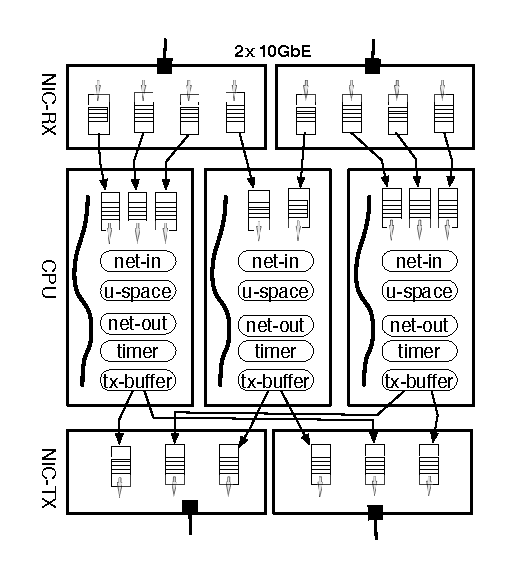
\includegraphics{figs/queues-cores.eps}
\centering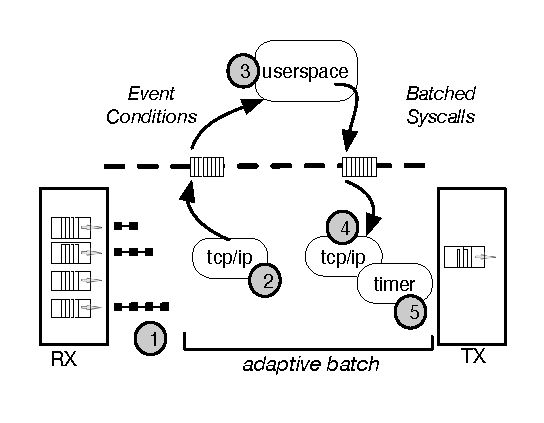
\includegraphics{figs/pipeline}
\caption{The IX pipeline.}
\label{fig:queues-cores}
\end{figure}

 

Fig.~\ref{fig:queues-cores} illustrates the run-to-completion
operation of elastic threads in the \ix dataplane. Each elastic thread
is associated with a specific set of receive queues from one or more
NICs. Each NIC uses RSS to implement flow-consistent hashing and
distribute incoming packets to queues. The queues are mapped in the
server's main memory and the NIC is given a set of buffer descriptors
that allow it to transfer incoming packets to memory using DMA\@.  The
elastic thread (1) polls the receive queues it is responsible for and
potentially posts fresh buffer descriptors to the NIC for use with
future incoming packets. The elastic thread (2) processes a bounded
number of packets through the TCP/IP networking stack, thereby
generating event conditions. Next, the elastic thread (3) passes
control to the user-space applications, which consumes all event
conditions. Assuming that the incoming packets include remote
requests, the application processes these requests and responds with a
batch of system calls. Upon return of control from user-space, the
elastic thread (4) processes all system calls, and in particular the
ones that direct outgoing TCP/IP traffic. It also (5) runs all kernel
timers in order to ensure compliant TCP behavior and (6) places
outgoing Ethernet frames in the NIC's descriptor rings for
transmission. Finally, it notifies the NIC to initiate a DMA transfer
for these frames by updating the transmit ring's tail register.
This process operates continuously in a loop until there are no
event conditions posted. In this situation, we enter a quiescent state, where
we periodically poll the receive queues and potentially engage
in power conservation states or yield to the control plane.

The \ix dataplane consists of 37K SLOC~\cite{url:sloccount}.  We leveraged existing
codebases in its development: 43\% is derived from the DPDK variant of
the Intel NIC device driver~\cite{intel:dpdk}, 23\% from the lwIP
TCP/IP stack~\cite{dunkels2001design}, and 16\% from the Dune library.
All three code bases are highly modified for \ix. The rest is
approximately 7K SLOC of new code. We chose lwIP as a starting point
for TCP/IP processing because of its modularity and its maturity as a
RFC-compliant, feature-rich networking stack. We implemented
RFC-compliant support for UDP, ARP, and ICMP.
% It allows us to be RFC-compliant for TCP, UDP, ARP, and ICMP.
Since lwIP was optimized for memory efficiency in embedded
environments, we had to radically change its internal data structures
for multi-core scalability and fine-grain timer management. We did not
yet optimize the lwIP code for performance. Hence, there is room for
improvement in the results shown in \S\ref{sec:eval}.



\subsection{Multi-core Scalability}
\label{sec:impl:cohfree}

The \ix dataplane is optimized for multi-core scalability as elastic
threads operate in a synchronization and coherence free manner in the
common case. This is a stronger requirement than lock-free
synchronization, which requires expensive atomic instructions even
when a single thread uses a particular lock in the common
case~\cite{DBLP:conf/sosp/DavidGT13}.  This was made possible 
through a set of conscious design and implementation tradeoffs. 

First, the \ix API is commutative. Events are processed independently
on each elastic thread. Handles identify flows but cannot be exchanged
between elastic threads. There is no file descriptor namespace.
According to the commutativity rule, system call implementations can
only be coherence-free if the API itself is
commutative~\cite{DBLP:conf/sosp/ClementsKZMK13}.

Second, the API implementation is carefully optimized.  Each elastic
thread manages its own memory pools, hardware queues, event condition
queue, and batched system call queue. No synchronization is required
to access any of them. The implementation of event conditions and
batched system calls benefits directly from the explicit, cooperative
control flow transfers between \ix and the application by the elastic
thread.  Since there is no concurrent execution by producer and
consumer, event conditions and batched system calls are implemented
without relying on lock-free synchronization primitives based
on atomics.

Third, the use of flow-consistent hashing at the NICs ensures that
each elastic thread operates on a disjoint subset of incoming TCP
flows. Hence, no synchronization or coherence occurs during the
processing of incoming requests for a server application. For client
applications with outbound connections, we need to ensure that the
reply is assigned to the same elastic thread that made the
request. Since we cannot reverse the Toeplitz hash used by RSS~\cite{url:rss}, we
simply probe the ephemeral port range to find a port number that
would lead to the desired behavior. Note that this implies that two
elastic threads in a client cannot share a flow to a server. % \edb{\sout{In
% \S\ref{sec:eval}, we show that \ix scales wells to hundreds of
% thousands of outgoing connections.}}
 
% ephemeral source port no longer form namespaces, which allows an \ix
% client to support millions of outgoing connections.


% \ix selects the source ephemeral port based on
% the requesting elastic thread. Since the Toeplitz hash function cannot
% be reversed, \ix simply probes the ephemeral range and computes the
% Toepliz hash until a match is found.  


\ix does have a small number of shared structures, including some that
require synchronization on updates.  For example, the ARP table is
shared by all elastic threads and is protected by RCU
locks~\cite{mckenney1998read}, Hence, the common case reads are
coherency-free but the rare updates are not.
%
\dm{Can you add a sentence about what constitutes a quiescent period
  for RCU garbage collection, given that this is a very non-Linux
  API?}

% Worth a paragraph break here, since reconfiguration is a big
% deal. -dm
\ix also requires
synchronization when the control plane reallocates resources between
dataplanes.  For instance, when a core is revoked from a dataplane,
the corresponding incoming queues must be assigned to another elastic
thread. Such events are rare because resource allocation happens in a
coarse-grain manner. Finally, the application code may include
inter-thread communication and synchronization. While using \ix does
not eliminate the need to develop scalable application code, it
ensures that there are no scaling bottlenecks in the system and
protocol processing code. 

%\subsection{Cooperative Flow Control}
\subsection{Security Model}
\label{sec:impl:coop}

%\adam{rename this section ``Security Design/Model'' ?}

The \ix API and implementation leads to a cooperative flow control
model between application code and the network-processing stack.  But
unlike user-level stacks that also expose networking behavior to user
code,
\dm{Can you say something more specific than networking behavior?
  Maybe something like ``unrestricted raw network access''?}
the \ix protection model makes few assumptions about application
behavior. A malicious or misbehaving application can only hurt
itself. It cannot corrupt the networking stack or affect other
applications.

The \ix dataplane and the application collaboratively manage
memory. To enable zero-copy operation, a buffer used for an incoming
packet is passed read-only to the application, enabling zero-copy
operation. Applications that hold on to message buffers for extensive
periods of time must bound their use of this shared resource.  In the
transmit direction, zero-copy operation implies that the application
must not modify outgoing data
% maintain outgoing data immutable
until reception is
acknowledged by the peer. % \edb{\sout{If there is recepient is not
    % operating fast enough or there is network congestion, the sender
    % will soon experience memory pressure as well.}}

Since elastic threads in \ix execute both the network stack and
application code, a long running application can block further network
processing for a set of queues. This behavior in no way affects other
applications or dataplanes. We use a timeout interrupt to
detect elastic threads that spend excessive time in user mode (e.g.,
in excess of 10ms). We mark such applications as non-responsive and notify
the control plane. %\edb{\sout{to potentially take resource allocation actions.}}

Note that all application code in \ix runs in user-mode, while the
dataplane code is in protected ring 0. Applications cannot access
kernel memory, except for read-only message buffers, or network
hardware.  No sequence of batched system calls or other user-level
actions can be used to violate correct adherence to TCP and other
network specifications.  Furthermore, the dataplane can be used to
enforce network security policies (e.g., iptables or Amazon Security
Groups~\cite{url:amazon-sg}) or to implement the network virtualization functions typically
done in a hypervisor~\cite{nsdi:nsx}. Our security model is as strong
as conventional network stacks in commodity OSes and is missing from all
the recently proposed user-level networking stacks.

Our current implementation does not utilize an IOMMU: we entrust
the \ix kernel into the trusted code base by giving access to
descriptor rings with host-physical addresses to avoid the possible
performance overheads of using IOMMUs~\cite{iommu_overhead}.  This
decision is not fundamental to our design, and does not extend to
applications.

%Our current implementation does not yet utilize IOMMUs. As a result, a
%dataplane could potentially corrupt control plane memory through stray
%DMA operations. However, unlike user-level network stacks we do not
%strickly require IOMMU support, as untrusted application code is never
%s given direct access to NIC DMA engies. Rather, adding IOMMU support
%would improve security by creating a layer of in depth defense between
%dataplanes and control planes, possibly at the expensive of some
%performance overhead~\cite{iommu_overhead}.

\dm{This raised a couple of questions for me.  First, is the
  immutability of transmit buffers enforced by memory protection, or
  just by convention.  In other words, can you cause TCP segments to
  be sent with bad checksums or otherwise shoot yourself in the foot
  by writing to buffers in the send queue?  Second, why are message
  buffers read-only (or does this exclude the actual payload part).
  For example, if I'm implementing an HTTP proxy, can I make small
  modifications to a message buffer I just received and then
  retransmit it?  Or is the point that one would use scatter gather IO
  for such surgical edits?}


\section{Evaluation}
\label{sec:eval}

We evaluate the scalability of \ix and compare it to the Linux
baseline running a 3.11.10 kernel, and whenever possible to mTCP.  We
selected mTCP as it is the state-of-the-art user-space TCP alternative
available on the same hardware~\cite{jeong2014mtcp}.  We first
describe the experimental setup (\S\ref{sec:eval:setup}).  We then
characterize the performance using a series of micro-benchmark: the
popular NetPIPE ping-pong test~\cite{snell1996netpipe}
(\S\ref{sec:eval:netpipe}); the short message transaction test
previously used to evaluate MegaPipe and mTCP
in~\cite{han2012megapipe,jeong2014mtcp} (\S\ref{sec:eval:short}); and
the scalability of the system for large persistent connections
(\S\ref{sec:eval:scale}).  Finally, we characterize the performance of
the \ix system by running memcached -- a real-world massively deployed
application (\S\ref{sec:eval:memcached}).


\subsection{Experimental setup}
\label{sec:eval:setup}

Our experimental setup consists of a cluster of 19 clients and one
server connected by an HP 5820AF-24XG 10GbE switch.  The client
machines are a mix of dual Xenon E5-2637 running at 3.5 Ghz and single Xenon E5-2650 running at 2.6 Ghz with a single, Intel
82599EB 10GbE NIC connecting to the switch.  The server is a dual-Xeon E5-2665
running at 2.4 Ghz with 256 GB of DRAM with four Intel 2P X520 NICs.  Each
socket (client or server) has 8 cores and 16 hyperthreads.  When
reporting multi-core scalability, we report results with
hyperthreading enabled, and both hyperthreads of the cores are used.

For our experiments, the server is connected to the switch via either
a single 10GbE link or via a 4x10GbE bond configured as a L2+L3 hash.
Jumbo frames are never enabled.  Our
baseline configuration in each machine is the Ubuntu 12.04.4 LTS
distribution running the 3.11.10 Linux kernel.  Although the server
has two sockets, our experiments use only the CPU and memory resources
of the socket to which the NIC are attached.  
\edb{CONTREVERSIAL: We made this deliberate decision to eliminate NUMA
  imbalances from our experiments, and to most closely reproduce the
  setup used in ~\cite{jeong2014mtcp}}

%\christos{We should organize the eval in the following way: first
%  micro-benchmarks that showcase each of the advantages (high packet
%  rate, low latency/jitter, high connection/churn). The title of the
%  subsection should indicate the aspect evaluated. Then there should
%  a subsection on full app eval (memcache hopefully).}

\begin{figure}
\begin{centering}
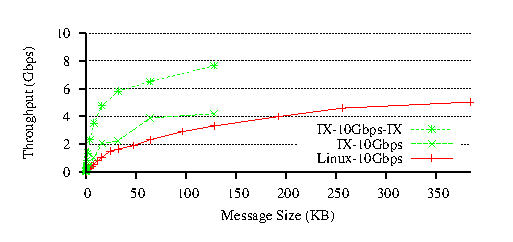
\includegraphics{figs/pingpong.eps}
\caption{NetPIPE performance for varying message sizes and system software configurations.}
\label{fig:pingpong}
\end{centering}
\end{figure}


%
%%%
%%%  use the ping-pong test to measure the half rountrip latency @ 64B
%%% 

\begin{table}[b]
\vspace{-1em}
\begin{center}
\begin{small}
\begin{tabular}{|l|c|c|}
\hline
Workload &  Avg lat. & 99\% lat. \\
\hline
Linux(base)-Linux(base)  & 60\microsecond & 0\microsecond\\
Linux(opt)-Linux(opt)    & 0\microsecond &  0\microsecond \\
mTCP-mTCP                & 0\microsecond &  0\microsecond \\
Linux(opt)-\ix           & 0\microsecond &  38\microsecond\\
\ix-\ix                  & 0\microsecond &  0\microsecond\\
\hline
\end{tabular}
\caption{Netpipe half-roundtrip latency (s=64B)}
\vspace*{-2em}
\label{tbl:pingpong}
\end{small}
\end{center}
\end{table}




%% put the key last to have correct numbering

\begin{figure*}[t]

\centering
  \vspace*{0.3in}
 \subfloat[Multi-core scalability (n=1;s=64B)]{
  \label{fig:short:mcore}
   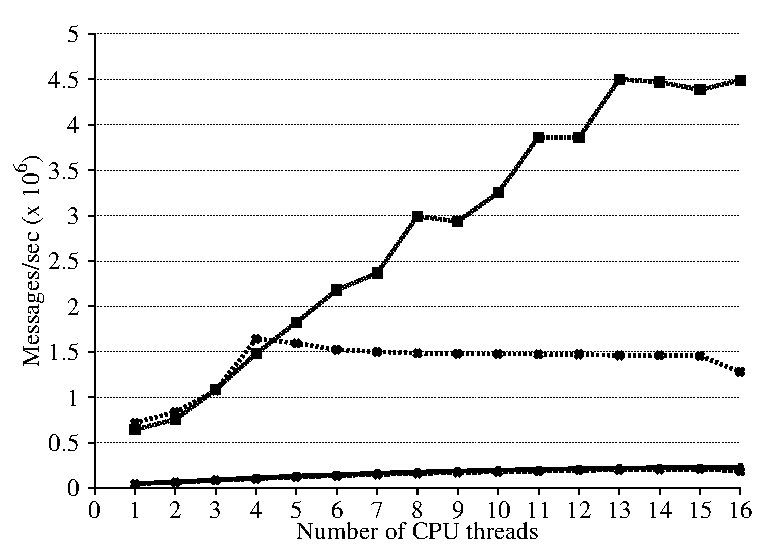
\includegraphics{figs/short-mcore.eps}}
 \hspace{.01in}
 \subfloat[$n$ roundtrips per conn. (core=8,s=64B)]{
  \label{fig:short:roundtrips}
  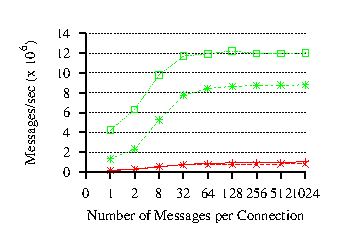
\includegraphics{figs/short-roundtrips.eps}}
  \hspace{.01in}
 \subfloat[Different message sizes $s$ (core=8,n=1)]{
  \label{fig:short:size}
  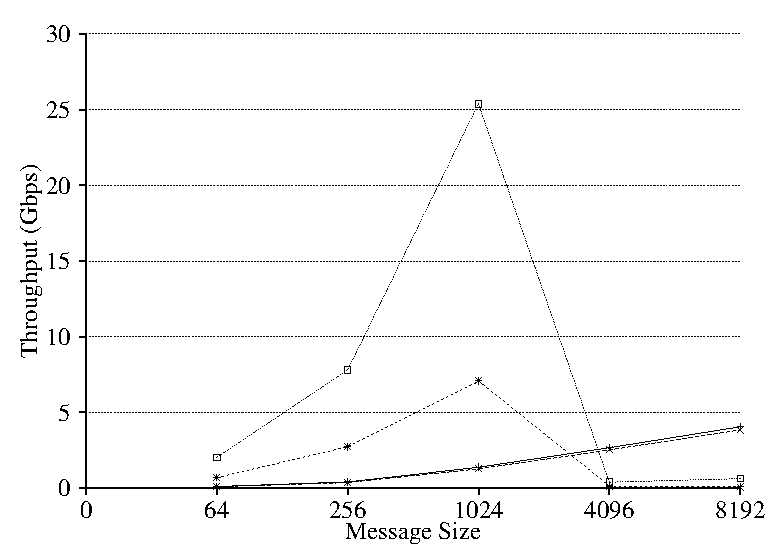
\includegraphics{figs/short-size.eps}}
 \centering
  \vspace{-1.9in}
  \subfloat{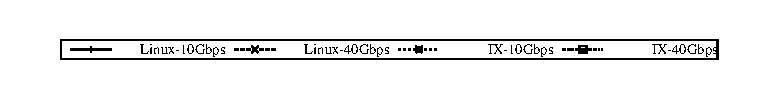
\includegraphics{figs/short-key.eps}}
 \vspace{1.5in}
 \
\caption{Short message performance.}
 \label{fig:short}

\end{figure*}


Whenever both practical and relevant, we compare the performance of an
\ix server with both the baseline Linux configuration and with mTCP, a
recently-published user-level TCP stack specifically designed for
scalability~\cite{jeong2014mtcp}.  Unless specifically mentioned, all
clients run the same Linux configuration. 

The Linux server implementations use the \texttt{libevent} framework
running on XXX threads to serve the clients, and the \texttt{epoll} system call. The mTCP server
implementation use the native mTCP API running on up to 8 cores
(within each core, one hyperthread is dedicated to processing the
network stack).  We downloaded and installed mTCP
from the public-domain implementation~\cite{url:mtcp}, but re-wrote the
benchmarks as they were not part of the distribution.  To run mTCP, we
switch to a kernel-2.6.36, as this is the most recent supported kernel
version.
Finally, \ix server use
the native \ix API running on up to 8 cores (using symmetrically both
hyperthreads).  For all experiments, we use the same Linux client code, generally also written using \texttt{libevent}.


\subsection{High-bandwidth and low-latency}
\label{sec:eval:netpipe}


We start the evaluation with the popular NetPIPE ping-pong
benchmark~\cite{snell1996netpipe} that exchanges a fixed-size message
between two servers.  The benchmark is used to calibrate the latency
and single-flow bandwidth of a communication link: with minimal
message size (64B), this benchmark determines the one-way latency for
short message communication.  With increasingly larger messages, it
determines how quickly this single ping-pong behavior can utilize 50\%
of the available bandwidth on the link.


Fig.~\ref{fig:pingpong} compares the performance of various
configurations for different message sizes.  As expected, the
bandwidth increases with the message size, and rises to half of the
maximum bandwidth with messages as small as 32KB for \ix-\ix.  In
constrast, both Linux-Linux and mTCP-mTCP lag and only reach the
half-bandwidth mark with messages sizes of 384KB and 1MB,
respectively.  

The difference is also noticeable with small message sizes, in
particular with 64B payloads.  The one-way latency is 6.8\microsecond
between two machines running \ix, 24\microsecond if they are running
Linux, and 80+XXX\microsecond if they are running mTCP.  The
difference in system architecture help explain such a dramatic
difference: \ix has a dataplane model that polls queues and runs them
to completion; Linux has an interrupt model, which wakes up the
blocked process.  The mTCP authors mention high context switching
overheads between the various threads in their architecture, and the
need for aggressive batching~\cite{jeong2014mtcp}, which helps explain
why it is such a challlenging benchark for that system\footnote{Our HP
  switch is well-amortized by now, which likely impacts performance;
  we performed the same benchmark on a current, low-latency Arista
  switch and measured XXX 5.6\microsecond between a pair of comparable
  (but not identical) servers both running \ix. We have a low-latency
  switch on order that will be used for the results of the
  camera-ready.}.

\subsection{Handling high TCP connection churn}
\label{sec:eval:short}


We then evaluate \ix's multi-core scalability in handling workloads
with extreme connection churn by using the same benchmark used to evaluate
Megapipe~\cite{han2012megapipe} and mTCP~\cite{jeong2014mtcp}:
multiple clients connect to a single server listening on a single
port, send a request of size $s$ and wait for an echo of a message of
the same size.  As with NetPIPE, while accepting the message, the server holds off its
echo response until the message has been entirely received.
Each client performs this synchronous remote procedure
call $n$ times, and then close the connection using a reset
(\texttt{TCP RST}).


\edb{PLACEHOLDER:} Fig.~\ref{fig:short} shows the results for both
10GbE and 4x10GbE hardware configurations.  We first
are able to confirm and reproduce the mTCP performance published in
~\cite{jeong2014mtcp}.  On this benchmark, \ix generally scales XXx
better than mTCP on a per core basis and XXx better than Linux.  In
Fig.~\ref{fig:short:mcore}, we see that \ix can saturate the single
10Gbpe wire using only 3 cores; in contrast mTCP requires all 8
cores. \ix can further scale to nearly XX\% of the wire limit on a
4x10GbE configuration, and using a single socket.
Fig.~\ref{fig:short:roundtrips}, which uses 8 cores, similarly shows
that \ix can nearly saturate the wire on the single-link
configuration, but remains CPU-bound on the 4x10 configuration.
Finally, Fig.~\ref{fig:short:size} shows that only \ix can saturate
4x10Gbps with 4KB messages, and only \ix and mTCP can saturate the
single-link configuration.


\subsection{Connection Scalability}


%FIXME if different keys


\begin{figure*}[t]

\centering
  \vspace*{0.3in}
 \subfloat[Throughput for varying established connections]{
  \label{fig:connscaling:throughput}
   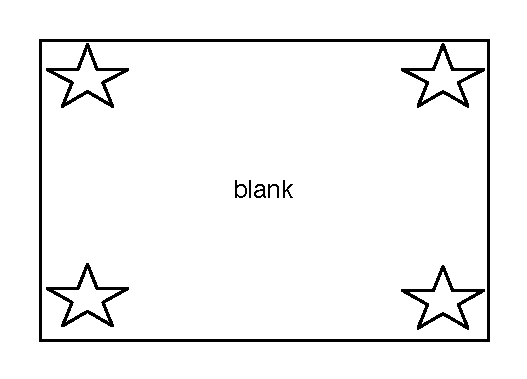
\includegraphics[width=.49\textwidth,clip]{figs/blank.eps}}
 \hspace{.02in}
 \subfloat[Avg. and 99\% latency for varying established connections]{
  \label{fig:connscaling:lat}
  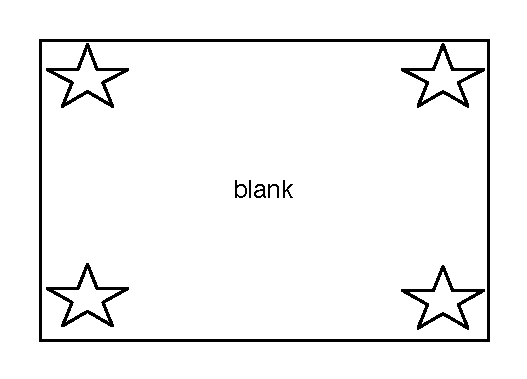
\includegraphics[width=.49\textwidth,clip]{figs/blank.eps}}
\centering
  \vspace{-2.8in}
  \subfloat{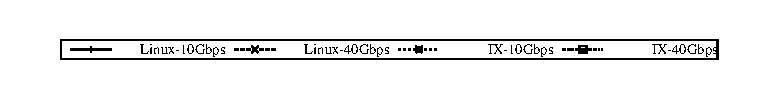
\includegraphics[width=1\textwidth,clip]{figs/short-key.eps}}
 \vspace{2.3in}
 \
\caption{Connection scaling}
 \label{fig:connscaling}

\end{figure*}


\label{sec:eval:scale}

We now evaluate \ix's scalability when handling a large number of
concurrent connections. In this benchmark, each client machine runs
$n$ threads, with each thread independently performing a 64B remote
procedure call to the server.  Each RPC randomly chooses among $m$
open sockets to perform the RPC.  In our setup with 19 clients, the
server must multiplex among $19 \times n \times m$ open connections.
We experimentally set $n \leq 24$ to maximize throughput.  We report
the maximal throughput in messages per second for varying number of
total established connections.

Fig.~\ref{fig:connscaling} shows the results.  As expected, throughput
increases with the degree of concurrency, but then decreases with
increasing number of connections due to the increasingly high cost of
multiplexing among open connections.  At the peak, \ix performs XXx
better than Linux, consistent with the results from
Fig.~\ref{fig:short:roundtrips}.  With 100,000 connections, \ix is
able to deliver XX\% of its peak throughput, whereas Linux only
delivers XXX\% of its own peak throughput\footnote{Unexplained
  performance issues with our client configuration setup limit our
  experiments to 100,000 connections at the time of submission. \ix is
  designed to scale to millions of concurrent connections.}


\subsection{Application performance -- memcache}
\label{sec:eval:memcached}

\begin{figure*}
\begin{centering}
\subfloat[Latency vs throughput for the memcached ETC workload.]{
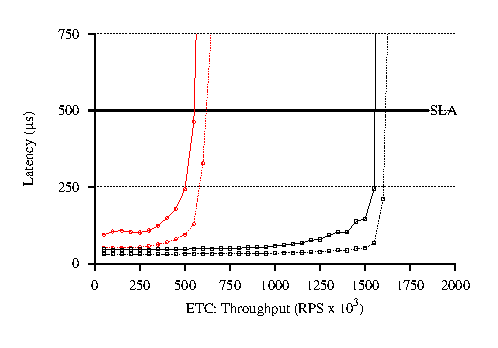
\includegraphics{figs/memcached-etc-basic.eps}}
\subfloat[Multilate-Me Again!]{
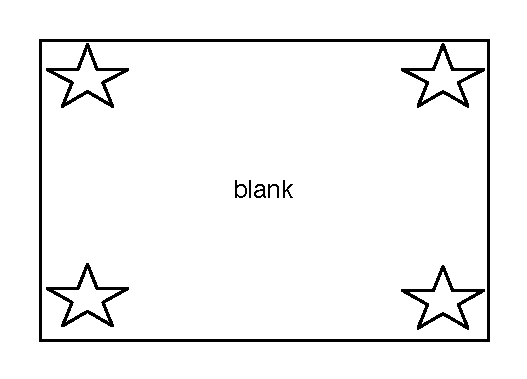
\includegraphics{figs/blank.eps}}
\caption{Capacity and quality of service of memcached on Linux and \ix for XXX and YYY concurrent, established connections}
\label{fig:mutilate}
\end{centering}
\end{figure*}



We now validate the performance benefits of the protected dataplane
design on memcached -- a real world, massively deployed, in-memory
key-value store built on top of the libevent framework.  We use the
mutilate~\cite{url:mutilate} load-generator and tool to measure
average and 99\% latency as a function of the throughput delivered by
the server~\cite{Leverich:RHSU:2014}.

Fig.~\ref{fig:mutilate} reports the latencies as a function of the
number of queries per second.  The peak QPS is measured using \ix at
XXX, which maps to a bandwidth leaving the server of XXX Gbps, or XX\%
of the theoretical wire rate of the machine.  We report the numbers
for Linux and \ix for XXX and YYY established, concurrent
connections served by the 18 clients.

Our results show that \edb{TODO}.....

\subsection{Web serving performance}


\todo Benchmark: lightttpd -- used by Affinity-Accept and mTCP.  

\todo ngnx: an actually used webserver.


%%%%%
%%%%% very optimistic
%%%%%

%
\subsection{Multi-tier Performance}

\edb{THIS IS A STRECH STRETCH GOAL} 

Evaluating the performance of a highly-scalable, multi-tier
environment in a lab environment is challenging on multiple fronts:
first, there are ---to the best of our knowledge--- no universally
accepted multi-tier benchmarks that involve key-value stores and in
general that are representative of web-scale applications.  Second,
most lab enviornments are orders of magnitude smaller than a
datacenter.

Therefore, we construct a simple, synthetic multi-tier benchmark that
mimics the behavior of a social application stored in an in-memory
key-value store.  The application is a simple \texttt{http} server
that returns the top-most recent update among a users list of friends.
The application server parses the http request to
get the userid, uses the user id to return a friends-list from a
key-value store, and then queries the key-value store individually for
each friend for the most recent value.  It then processes replies and
return the top-most entries.  In our experiments, we model a database
with $10^7$ million users, each with 100 friends. 

We scale the benchmark to model a cluster deployment with $\alpha$
client connections per application server, $\beta$ httpd and $\gamma$
memcached servers.  Keys are distributed uniformly between the
$\gamma$ servers.  We model a large-scale deployment with
$\alpha=10^5$, $\beta=10^4$ and $\gamma=10^4$ on a deployment that consists of 4
actual application servers and 1 memcached server (running on our
server hardware with 4x10GbE connectivity).  Each application server
runs \texttt{lighthttpd} with the application logic written directly
within the server, and maintains a distinct connection for each of the
$\alpha$ virtual clients and $\gamma$ virtual nodes.  The key-value store is
running \texttt{memcache} as described in \S\ref{sec:eval:memcache}.
We use the remaining 14 client machines to simulate $4 \times \alpha$
clients and the 19th client to measure the latency of the application.

Fig.~\ref{missing} reports the latency as a function of the
throughput, as determined by varying the client load.  We compare a
Linux baseline with one in which \ix is used to run both the
application server and the memcached server.  We note that the choice
of operating system on the application server determines the number of
concurrent connections. Indeed, because of the coherence-free
execution model, each application server needs to open a distinct TCP
flow to the same virtual node for each of its hardware threads.

\edb{OPTIMISTIC: } Fig.~\ref{missing} shows that \ix can saturate the
hardware connectivity.  Indeed, the bottlneck consits of the
communication 







\section{Discussion}
\label{sec:disc}


\myparagraph{What makes \ix faster:} The results in \S\ref{sec:eval}
show that a networking stack can be implemented in a protected OS
kernel and still deliver wire-rate performance for most benchmarks.
The tight coupling of the dataplane architecture, using only a minimal
amount of batching to amortize transition costs, causes application
logic to be scheduled at the right time, which is essential for
latency-sensitive workloads.  Therefore, the benefits of \ix go beyond
just minimizing kernel overheads. Similar to
Exokernel~\cite{DBLP:conf/sosp/EnglerKO95}, the lack of intermediate
buffers pushes all abstractions outside of the OS kernel, allowing for
efficient, application-specific implementations.  In particular, the
zero-copy approach helps even when the user-level libraries add a
level of copying, as it is the case for compatibility interfaces in
our event library.  The extra copy occurs much closer to the actual
use, thereby increasing cache locality.  Finally, we took great care
in tuning the implementation of \ix for multi-core scalability,
eliminating constructs that introduce synchronization or coherence
traffic.

\myparagraph{Using interrupts as a fallback:}
\edb{ALT. TO NEXT PAR.} 
The security model of \ix assumes some cooperation from applications,
specifically to handle events in a quick, non-blocking manner;
operations with extended execution times are expected to be delegated
to background threads rather than execute within the context of
elastic threads.  The \ix dataplane is designed around polling, with
the provision that interrupts can be configured as fallback
optimization to refresh receive descriptor rings when the ring is
nearly full and to refill the transmit queues when it is empty (step
(1) and (6) in Fig~\ref{fig:dataplane}).  Timer interrupts exist
primarily to detect runaway elastic threads and guarantee resource
revocation.


\myparagraph{Using interrupts as a fallback:} Some applications
service requests that require extended intervals of
compute time. We intend for these requests to be delegated
to background threads rather than elastic threads in order
to ensure that elastic threads remain responsive.
However, \ix could also be modified to better tolorate
unanticipated delays during application processing in elastic threads.
One option would be to use interrupts as a fallback mode. On the receive side, we
could program the NIC to fire an interrupt whenever the
recieve descriptor ring is almost full. The dataplane could
then move packets from the receive ring to a structure in software, averting
buffer underrun. On the transmit side, we could program
the NIC to fire an interrupt whenever the transmit ring becomes
empty so that it can be refilled. Such an interrupt would only need
to be armed when there is additional transmit data pending. A desirable
property of this approach is that neither interrupt would
be triggered as long as elastic threads are sufficiently responsive,
but if an elastic thread misbehaves, the \ix dataplane would
be able to regain control and catch up on network processing.


%\myparagraph{Hardware Bottlenecks:} We achieved very high packet
%rates with \ix, often saturating the bandwidth limit of our 10 GbE NIC.
%One unexpected performance bottleneck was the NIC and its DMA engine.
%We discovered that minimizes register writes was an effective optimization.
%\adam{finish this section}


\myparagraph{Subtleties of adaptive batching:} All experiments of
\S\ref{sec:eval} were conducted with a maximal batch size of $B=64$
packets per iteration. In exploring the impact of the batch size, we
first confirmed the intuition that smaller values of $B$ reduce tail
latency.  Fig.~\ref{fig:batch} compares the throughout of a CPU-bound
microbenchmark for different values of B, and shows that batches as
low as $B=32$ can deliver maximal throughput for this workload.
However, we ran into unexpected limitation of adaptive batch when
running \ix at high packet rates, on many cores, and with small
average batch sizes: the high rate of PCIe writes required to post
fresh descriptors at every iteration lead to overall degraded
performance as we added cores to \ix.  To avoid the problem, we simply
coalesced PCIe writes on the receive path so that we replenished at
least 32 descriptor entries at a time.  Luckily, we did not have to
coalesce PCIe writes on the transmit path as that would have impacted latency.



\myparagraph{Limitations of current prototype:} The current prototype
supports any stateless offload NIC with multiple queues and RSS
support. \edb{REDO\sout{The NICs we currently use support RSS group of 16 queues,
which is inadequate given current multi-core trends}}. Nevertheless, the
trend in NICs seems to be towards support for larger number of
queues~\cite{radhakrishnan2014senic}. We also plan to explore using Intel's Flow
Director~\cite{intel:82599} to provide connection
affinity~\cite{DBLP:conf/eurosys/PesterevSZM12} as an alternative to
our current flow hashing implementation. Our current implementation
does not exploit IOMMUs or VT-d. Instead, it uses Dune to map
descriptor rings directly into \ix memory as a form of
paravirtualization~\cite{DBLP:conf/sosp/BarhamDFHHHN03}.  Although
this choice puts some level of trust into \ix, the applications remain
securely isolated.

\myparagraph{Future work:} This paper focused on the \ix dataplane
design. \ix is designed and implemented to support the dynamic
addition and removal of elastic threads in order to achieve energy
proportional and resource efficient computing. So far we have tested
only static configurations. In future work, we will design a dynamic
runtime that rebalances hardware queues between available elastic
threads in a manner that maintains throughput and latency constraints.
%
We will also explore the synergies between \ix and networking
protocols designed to support microsecond-level latencies and reduced
buffering characteristics of \ix deployments such as
DCTCP~\cite{DBLP:conf/sigcomm/AlizadehGMPPPSS10} and
ECN~\cite{ramakrishnan2001addition}. Finally, we will investigate \ix
implementations of alternative APIs, such as
MegaPipe~\cite{DBLP:conf/osdi/HanMCR12}, cooperative
threading~\cite{DBLP:conf/sosp/BehrenCZNB03}, and rule-based
models~\cite{DBLP:conf/hotos/StutsmanO13}.




\section{Discussion}

\christos{I think these issues should be discussed within the
  implementation and eval sections}
\todo Lessons learned: importance of hardware knobs and micro-architectural effects.

\todo libevent compatibility

\todo Use of dataplane vs. virtual machines. 

\section{Related Work}

We organize the discussion topically, while avoiding redundancy with
the commentary already exposed in \S\ref{sec:motivation:current}.


\myparagraph{Separation of control and data plane:} The notion of
architected separation between control and data plane is pervasise in
the design of networking protocols and devices.  In systems,
virtualization also separates the control and execution functions. For
example, a type-2
hypervisors~\cite{DBLP:journals/tocs/BugnionDRSW12,misc/kivity07kvm}
use a Linux environment for control, and a separate virtualization
module for execution.  We leverage Dune and the same virtualization
hardware to run the \ix as a process of the control plane.
Arrakis~\cite{peter2013arrakis,arrakisTR13} recently proposed to
separate the networking stack into a distinct dataplane.  Our work
most closely ressembles Arrakis, but with noticeable differences:
first, Arrakis uses the Barrelfish multikernel as its control plane
and run-time layer, whereas the \ix control plane runs on a vanilla
Linux foundation.  Second, Arrakis runs its own, homegrown, networking
stack at userlevel, whereas \ix uses runs its networking stack
protected from the application.

\myparagraph{User-level networking stacks:} Our work shares the same
motivation as mTCP~\cite{jeong2014mtcp} in providing highly-scable
networking stack for web-scale applications, including in the presence
of high connection count and churn.  Both also focus on bounding the
latency of RPC, and were designed to use the same standard Intel NIC.
mTCP has an asymmetrical model where the first hyperthread of each
core runs the networking stack and the second one the application.
Also, the application and networking stack share the same address
space without protection.  \ix can use both hyperthreads symmetrically
and protects the protocol stack.  \edb{PLACEHOLDER:} Our results show
that, for the same workloads, \ix typically outperforms mTCP by 3x on
CPU-bound workloads, and provides lower latency.
 
\myparagraph{Hardware and protocol specialization:} Our work applies
specialization in software to commodity servers and networking
equipment.  Although our work shows that latencies and jitter can be
substantially reduced, on the same hardware, by using \ix rather than
standard Linux stacks or even userlevel stacks, we are still outside
of the latency range enabled by specialized adapters that expose RDMA
directly to applications.  Commercial Infiband RDMA adapters offer
RDMA and remote procedure calls in
$1-3$\microsecond~\cite{DBLP:conf/sosp/OngaroRSOR11,Jose:2011:MDH,mitchell:rdma,dragojevic14farm}.
Our current evaluation of \ix suggests that there is still room for
improvements.  Indeed, on the same hardware, we've measured UDP
one-way latencies that were a fraction of the NetPIPE latencies,
suggesing that the TCP codebase could be substantially optimized in
future work.

\myparagraph{Asynchronous and zero-copy interactions:}
Many systems address the system interaction limitations of the POSIX
model, and in particular inability to batch requests across sockets,
For example, mTCP~\cite{jeong2014mtcp},
MegaPipe~\cite{han2012megapipe} and NetMap~\cite{rizzo2012netmap} all
use some shared memory queue or ring for communication between the
networking stack and the application.  The queue or ring is required
because of the asynchronous execution of the two components.  In
contrast, \ix uses an array mechanisms and an interleaved execution
model, which enables coherence-free execution.  The semantics of POSIX
sockets also prevent non-blocking, zero-copy transfer of data. Systems
such as IO-lite~~\cite{DBLP:journals/tocs/PaiDZ00} use memory
protection mechanisms to unify buffering.  \ix enables a zero-copy
model: on receive, it relies on memory protection to safely expose
incoming packets to application; on send, \ix explicitely notifies the
application when the data has been acknowledged by the peer.



\paragraph{Adaptive, batched run to completion}

\todo TODO

\paragraph{Coherence-free, flow-consistent processing}

\todo Affinity Accept, mTCP, ...

\paragraph{Buffering at the NIC edge}

\todo DCTCP (actually belongs there?)


\paragraph{Improvements to existing operating systems.}

\paragraph{API design.}


\paragraph{Hardware specialization - Dataplanes.}

\paragraph{Operating system architecture.}

\paragraph{Domain-specific and library operating systems.}

\subsection{Misc. to cite}

Stuff to cite (that is not otherwise cited) ... that we should either incorporate or drop:


\begin{itemize}

\oldcite{Alizadeh DCTCP}{DBLP:conf/sigcomm/AlizadehGMPPPSS10}
\oldcite{Libra JVM}{DBLP:conf/vee/AmmonsABSGKKRHW07}
\oldcite{Scheduler activations}{DBLP:journals/tocs/AndersonBLL92}
\oldcite{Atikoglu - Workload analysis fo large-scale key-value store}{Atikoglu:2012:WAL}
\oldcite{Basu - Efficient virutal memory for big memory servers}{DBLP:conf/isca/BasuGCHS13}
\oldcite{Multikernel}{DBLP:conf/sosp/BaumannBDHIPRSS09}
\oldcite{RadixVM}{DBLP:conf/eurosys/ClementsKZ13}
\oldcite{TCP Onloading}{DBLP:journals/cacm/DeanB13}
\oldcite{Unikernel - case for single app OS}{DBLP:conf/asplos/MadhavapeddyMRSSGSHC13}
\oldcite{Waldspurger - CPU balloning}{DBLP:conf/osdi/Waldspurger02}
\oldcite{Drepper - cost of virtualization}{DBLP:journals/queue/Drepper08}
\oldcite{Disco}{DBLP:journals/tocs/BugnionDGR97}
\oldcite{Salzer -E2E principle}{DBLP:journals/tocs/SaltzerRC84}
\end{itemize}



\section{Conclusion}

We described \ix, a dataplane operating system that leverages hardware
virtualization to separate and isolate the Linux control plane, the
\ix dataplane instances that implement in-kernel network processing,
and the network-bound applications running on top of it.  The \ix
dataplane provides a native, zero-copy API that explicitly exposes
flow control to applications. The dataplane architecture optimizes for
both bandwidth and latency by processing bounded batches of packets to
completion and by eliminating synchronization on multi-core
servers. On microbenchmarks, \ix noticeably outperforms both Linux and
mTCP in terms of both latency and throughput, scales to hundreds of
active concurrent connections, and can saturate 4x10GbE configurations
using a single processor socket.  Finally, we show that porting
\texttt{memcached} to \ix removes kernel bottlenecks and improves
throughput by up to \data{4.7}{4.1}$\times$.



%input{acks}


\bibliography{../common/dblp,../common/gscholar,../common/misc}
\bibliographystyle{abbrv} 

\ifcomments
\subsection{Misc. to cite}

XXX REMOVE ME XXX


Stuff to cite (that is not otherwise cited) ... that we should either incorporate or drop:


\begin{enumerate}

\oldcite{Alizadeh DCTCP}{DBLP:conf/sigcomm/AlizadehGMPPPSS10}
\oldcite{Libra JVM}{DBLP:conf/vee/AmmonsABSGKKRHW07}
\oldcite{Scheduler activations}{DBLP:journals/tocs/AndersonBLL92}
\oldcite{Atikoglu - Workload analysis fo large-scale key-value store}{Atikoglu:2012:WAL}
\oldcite{Basu - Efficient virutal memory for big memory servers}{DBLP:conf/isca/BasuGCHS13}
\oldcite{Multikernel}{DBLP:conf/sosp/BaumannBDHIPRSS09}
\oldcite{RadixVM}{DBLP:conf/eurosys/ClementsKZ13}
\oldcite{TCP Onloading}{openonload}
\oldcite{Waldspurger - CPU balloning}{DBLP:conf/osdi/Waldspurger02}
\oldcite{Drepper - cost of virtualization}{DBLP:journals/queue/Drepper08}
\oldcite{Thialfi}{DBLP:conf/sosp/AdyaCMP11}
\oldcite{Cavium Octeon}{cavium-octeon}
\oldcite{Fan 2013 Mem Cache 3}{fan2013memc3}
\oldcite{Case against userlevel networking}{magoutis2004case}

\end{enumerate}


\fi

%
\section{Internal notes}


\subsection{ CUT from Intro}



In addition, such applications must scale in terms of bandwidth and
concurrent connection counts, and ideally solve the \emph{C10M
  problem}~\cite{theC10Mproblem}: for a given server, scale to 10
million concurrent TCP connections, saturate 10 GbE interfaces, and
deliver 10~\microsecond latency (mean), with an additional latency
jitter of not more than an extra 10~\microsecond.  Today, million+
concurrent connections are desirable in Internet-facing notification
servers~\cite{DBLP:conf/sosp/AdyaCMP11} or messaging
servers~\cite{whatsapp-2mil}. 


\begin{comment}

%%% V1

We focus here on three high-level challenges for web-scale
applications that point to the need to address energy-proportionality,
connection scalability, and quality-of-service for web-scale
applications.

First, at the highest level, web-scale applications ideally deliver
the highest possible quality of service in the most
energy-proportional manner~\cite{DBLP:journals/computer/BarrosoH07}.
In practice, these two goals are often at odds with each other:
techniques that can improve quality-of-service, and in particular
reduce end-to-end latency, often consume much more energy.  For
example, low-power states save substantial amounts of energy, at the
cost of an increased latency measured in XXX when transitioning back
into a normal operating system.

Second, the nodes of web-scale applications are often characterized by
extremely high fan-out and high fan-in requirements.  An application
server may rely on tens of thousands of downstream services, and a
downstream service may serve hundreds of thousands of
clients~\cite{missing}.  At the extreme end of the spectrum,
notification and communication services must scale to the hundreds of
millions of Internet clients~\cite{DBLP:conf/sosp/AdyaCMP11}.
Unfortunately, existing implementations of the TCP/IP networking stack
in current systems were never designed to scale to such sizes.  As a
consequence, Facebook pragmatically chose to forgo the TCP protocol in
favor of connection-less UDP datagrams~\cite{nishtala2013scaling} for
its memcached implementation.  WhatsApp put significant engineering
efforts to tun FreeBSD to scale to 2 million concurrent
connections~\cite{whatsapp-2mil}.

Third, these high fan-in and fan-out applications suffer from the
\emph{long tail} problem, with the latency of the application
determined by the latency of slowest-responding
node~\cite{DBLP:journals/cacm/DeanB13}.  To lessen the impact of the
long tail, datacenter operators often overprovision servers to ensure
that they can operate at low utilization.

Collectively, the second and third challenge have been proposed as the
\emph{C10M problem}~\cite{theC10Mproblem}: for a given server, scale
to 10 million concurrent TCP connections, saturate 10 GbE interfaces,
and deliver 10~\microsecond latency (mean), with an additional latency
jitter of not more than an extra 10~\microsecond.  The conventional
wisdom is that such a solution must bypass the operating system
entirely.  For example, mTCP~\cite{jeong2014mtcp} is a user-level TCP
stack with the highest known scalability for short-lived connections.

\end{comment}


\subsection{Stuff to cite somehow}
\begin{itemize}


\item DPDK
\item IXGBE
\item some kind of user-mode zero-copy network driver, but I think it is proprietary. \url{http://www.ntop.org/products/pf_ring/}
\item same for FreeBSD \url{https://www.usenix.org/system/files/conference/atc12/atc12-final186.pdf}
\item mTCP - highly scalable userspace multicore TCP kernel~\cite{jeong2014mtcp}.  Site at \url{http://shader.kaist.edu/mtcp/}
\item Megapipe~\cite{han2012megapipe},
\item Affinity-accept~\cite{DBLP:conf/eurosys/PesterevSZM12}
\item Netmap~\cite{rizzo2012netmap}.
\item SO\_RESUEPORT (socket option).  
\item What's App 2milion socket post~\cite{whatsapp-2mil}
\item Dune~\cite{belay2012dune} ...
\end{itemize}

\subsection{Names and Concepts of IX}

\begin{itemize}
\item {\bf cpu}. A hardware thread, labelled x/y with x the core and y the HT
\end{itemize}


\subsection{To put in related work}

\paragraph*{Exokernel}   Exokernels~\cite{DBLP:conf/sosp/EnglerKO95} safely expose hardware to library operating systems.  We propose


\paragraph*{Akkaris}.  
Akkaris~\cite{peter2013arrakis} is the closest system.  It is
apparently built on the barrelfish multikernel~\cite{DBLP:conf/sosp/BaumannBDHIPRSS09} and uses VT-x
like Dune~\cite{belay2012dune}.

\paragraph*{Megapipe} 
Megapipe~\cite{han2012megapipe} proposes a high-performance socket
alternative for TCP/IP based applications for scalable network
applications.  Our API is inspired by it. This is similar to
Netmap~\cite{rizzo2012netmap}, which also ping shared buffers, but is
focused on libpcap applications.


\paragraph{mTCP}

MTCP is a user-level stakc (NSDI 2012) that outperform Megapipe and
Linux (w/ SO\_REUSEPORT) by large factors.  The design calls for a
userlevel TCP stack that runs in the same address space as the
application. The threading model calls for a 1:1 correspondance
between application threads and TCP threads, ideally running on the
two different hyperthreads of the same core.  This gives TCP threads
to run timers with high precision.  To offset the high cost of IPC,
mTCP relies on extensive batching of commands before waking the
distinct thread.  There is no protection between application and TCP
thread; a malicious (or owned) application can easily corrupt the TCP
protocol blocks and header space.  mTCP is built on top of the PSIO
engin, which provides an event-driven packet IO interface.

In constast, IX runs the TCP stack (in kernel model) and the
application on the same threads of control; an IX application can
therefore take advantage of all hyperthreads of the CPU (instead of
only half).  Furthermore, IX runs without any locks, lock-free data
structures, or atomic instructions, whereas mTCP relies on lock-free
data structures (which themsevles require atomic instructions).

mTCP does not expose the dual-thread model directly to
applications. Instead, it hides it behind a nearly-identical POSIX
variant (epoll --> mepoll).  IX exposes an event-driven API directly
to applications, via the libevent framework.

MTCP has some great design ideas that IX could/should leverage:

\begin{itemize}

\item Efficient timer management for high-socket count.  One bucket
  per remaining milisecond for near-term events, and an ordered list
  for longer-term events (TCP cleanup events).

\item They claim optimization for
short-lived connections, including the prioritization of SYN and ACK
packets on TX (which seems like a hack)

\end{itemize}

The evaluation of MTCP includes micro-benchmarks as well as basic
applications (ab + lighttpd, SSLshader).  Fig 7 shows the connection
setup/taredown throughput based on the number of cores, showing linear
speedup up to the measured 8 cores.  At 8 cores, they can setup, send
a 64B message and close a connection 150,000 times per second, using 8
cores (i.e. 16 threads).  They can actually accept/close 300,000
connections per second (Fig 8).

SSLsharer runs with up to 16K connections; they measure median and 95
percentile latency for response time.

They use the Jain index on a benchmark that downloads a 10MiB file
repeatedely across 8K connections to measure fairness.  8K is a small
number of connections.  Table 4 looks at the connection count and
thrhougput of WebReplay across 4x10GbE connections.  The workload
creates up to 15K connections per second and has up to 25k concurrent
connection (the text also mentions having up to 270,000 conurrent
connections).




\paragraph*{Kernel-bypass approaches}  Solarflare Openonload~\cite{openonload}, ...

\paragraph*{Containers}  Linux containers, BSD jail, ...


\paragraph*{Application-specific kernels}  
Exokernels had a bunch of them.
SplashOS~\cite{DBLP:journals/tocs/BugnionDGR97} proposed this in the
context of hypervisors (Disco).
Libra~\cite{DBLP:conf/vee/AmmonsABSGKKRHW07} was a JVM that ran
directly on top of Xen.  It Relied on a separate Linux VM to provide
networking and storage (like Azul).  The
Unikernel~\cite{DBLP:conf/asplos/MadhavapeddyMRSSGSHC13} (ASPLOS 13)
lays out the case for BaremetalOS because it lays out the case for
single app operating systems.  The Unikernel ported the Ocaml runtime
to run on top of Xen hypervisor (like libra).  Actually makes a case
for reduced latency jitter, at least in terms of thread scheduling -
I/O performance basically sucks though because still not taking
advantage of HW (uses Xen PV-NIC).

\section{Techniques and Concepts}

\paragraph*{The C10M problem} As stated by Robert Graham(?)~\cite{theC10Mproblem}.


\paragraph*{Scheduler activations} 
If apps are able to yield cores, and if apps are able to
asynchronously take advantage of new cores, scheduler
activations~\cite{DBLP:journals/tocs/AndersonBLL92} seem like a
perfect mechanism to make those cores available to other processes. 
The idea never really made it into POSIX, but we can use here because the API is different. 

\paragraph*{Ballooning}
Ballooing was introduced for memory
management~\cite{DBLP:conf/osdi/Waldspurger02}.  The balloon keeps
track of the amount of relinquished resources.  CPU ballooning could
be used to (i) start a max core pool, and (ii) dynamically resize it
according to the SLA and the global load.

\paragraph*{Virtual memory performance}  
Direct segment mapping~\cite{DBLP:conf/isca/BasuGCHS13} proposes to
replace the traditional TLB with a dedicated direct segment.
Drepper~\cite{DBLP:journals/queue/Drepper08} measured additional cost
of running workloads in virtualized domains due to two-dimensional
page walking.

\paragraph*{Latency distribution}  
Dean and Barroso~\cite{DBLP:journals/cacm/DeanB13} describe the
problems associated with tail latency in web-scale services.
Dynamo~\cite{DBLP:conf/sosp/DeCandiaHJKLPSVV07} talked about the
importance to evaluate key-value stores based on their 99.9\% latency.


\paragraph*{Commutativity and scalability} 
The scalable commutativy rule~\cite{DBLP:conf/sosp/ClementsKZMK13}
states that only commutative APIs can be implemented in a truly
scalable manner; our API and our implementation should support that.
RadixVM~\cite{DBLP:conf/eurosys/ClementsKZ13} provides scalable
address spaces for multithreaded applications; we address this as well.

\paragraph{The case against user-level networking}
Margo's original paper (same title)~\cite{magoutis2004case}

\paragraph*{Latency measurements}  

\section{Workloads}

\paragraph*{Memcached} 
Scaling memcached at Facebook~\cite{nishtala2013scaling} required
unnatural tricks such as relying on UDP and on in-network connection
proxies to compensate for the lack of scoket scalability of Linux.

Memcached is so important that folks are prototyping it in
FPGA~\cite{DBLP:conf/fpga/ChalamalasettiLWARM13}.  The authors's main evaluation is
that they can get comparable performance to an industry server with
10x the Performance/Watt, measured in KOPS/S/Watt (Table 3. memcached
``gets'' with 128B size data). To beat their numbers, we need to beat
30 Kops/sec/W to win.  Can we?  The comparison is a case of hardware
specialization vs. software specialization (of the OS).



\paragraph*{ngnx}
 % really old stuff



\end{document}

